\chapter{Algorithm}

This chapter presents all the passes which are applied to the code of the method until the final result is achieved.
Each pass is represented by a visitor which usually first collects information about the change that has to be made and
then alters the code.

\section{Renaming local variables to unique names}

This code transformation is needed in order to avoid name clashes later on, when the static nested class which
holds the variables potentially used after returning from a recursive call (both formal parameters and local variables)
is generated. The fields of this class will simulate the stack frame of the method.

The JVMS (Java Virtual Machine Specification)\abbrev{JVMS}{Java Virtual Machine Specification} states the
following\footnote{\url{http://docs.oracle.com/javase/specs/jvms/se8/html/jvms-2.html#jvms-2.6.1}}:

\begin{quote}
    The Java Virtual Machine uses local variables to pass parameters on method invocation. On class method invocation,
    any parameters are passed in consecutive local variables starting from local variable 0. On instance method invocation,
    local variable 0 is always used to pass a reference to the object on which the instance method is being invoked
    (\code{this} in the Java programming language). Any parameters are subsequently passed in consecutive local
    variables starting from local variable 1.
\end{quote}

In the context of this refactoring, the recursive call is defined only as a method call expression whose qualifier is
either absent or \code{this}, so the target reference of the instance method invocation never changes. This is why it is
not a field of the frame class. In the case of class method invocations, there is no target reference (\code{this}).

JLS specifies that\footnote{\url{https://docs.oracle.com/javase/specs/jls/se8/html/jls-6.html#jls-6.4}}:
\begin{quote}
    It is a compile-time error if the name of a formal parameter is used to declare a new variable within the body of
    the method, constructor, or lambda expression, unless the new variable is declared within a class declaration
    contained by the method, constructor, or lambda expression.

    It is a compile-time error if the name of a local variable v is used to declare a new variable within the scope of
    v, unless the new variable is declared within a class whose declaration is within the scope of v.
\end{quote}

This means that all the names of formal parameters and local variables whose scopes overlap are unique in the method
body. In other words, a compile-time error occurs for the program in
\labelindexref{Figure}{img:attempted-shadowing-of-a-local-variable}, but not for the program in
\labelindexref{Figure}{img:no-shadow}.

%\fig[width=4in]{src/img/attempted-shadowing-of-a-local-variable.png}{img:attempted-shadowing-of-a-local-variable}{Attempted shadowing of a local variable}
%\fig[width=4in]{src/img/no-shadow.png}{img:no-shadow}{Two non-overlapping scopes}
\begin{figure}[htb]
    \centering
    \begin{minipage}[b]{0.45\textwidth}
        \centering
        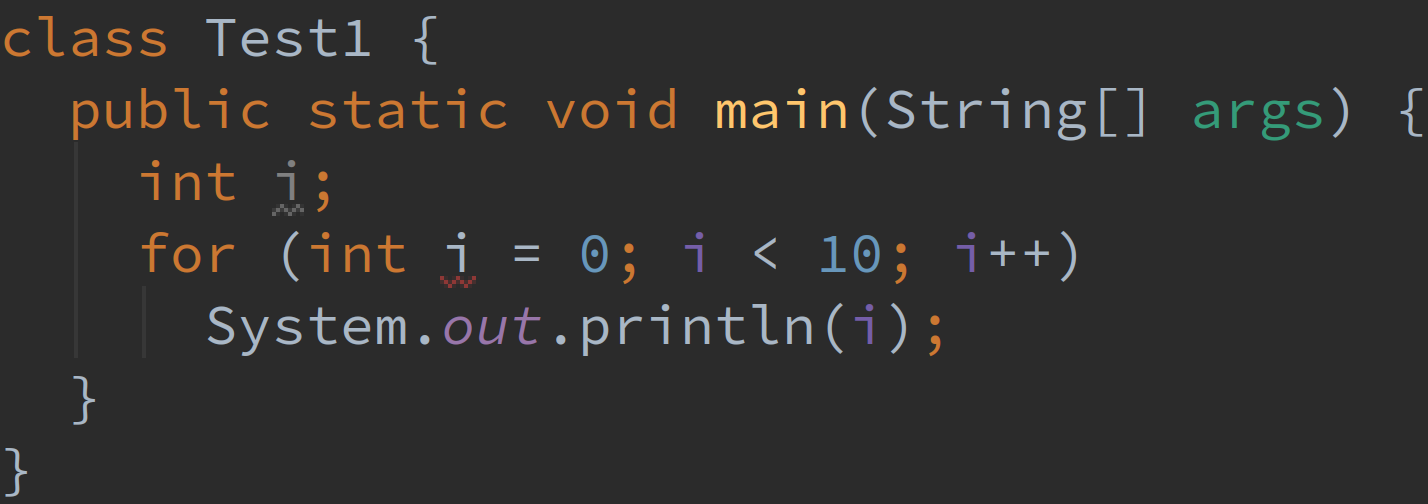
\includegraphics[width=\textwidth]{src/img/attempted-shadowing-of-a-local-variable.png}
        \caption{Attempted shadowing of a local variable \label{img:attempted-shadowing-of-a-local-variable}}
    \end{minipage}
    \hfill
    \begin{minipage}[b]{0.45\textwidth}
        \centering
        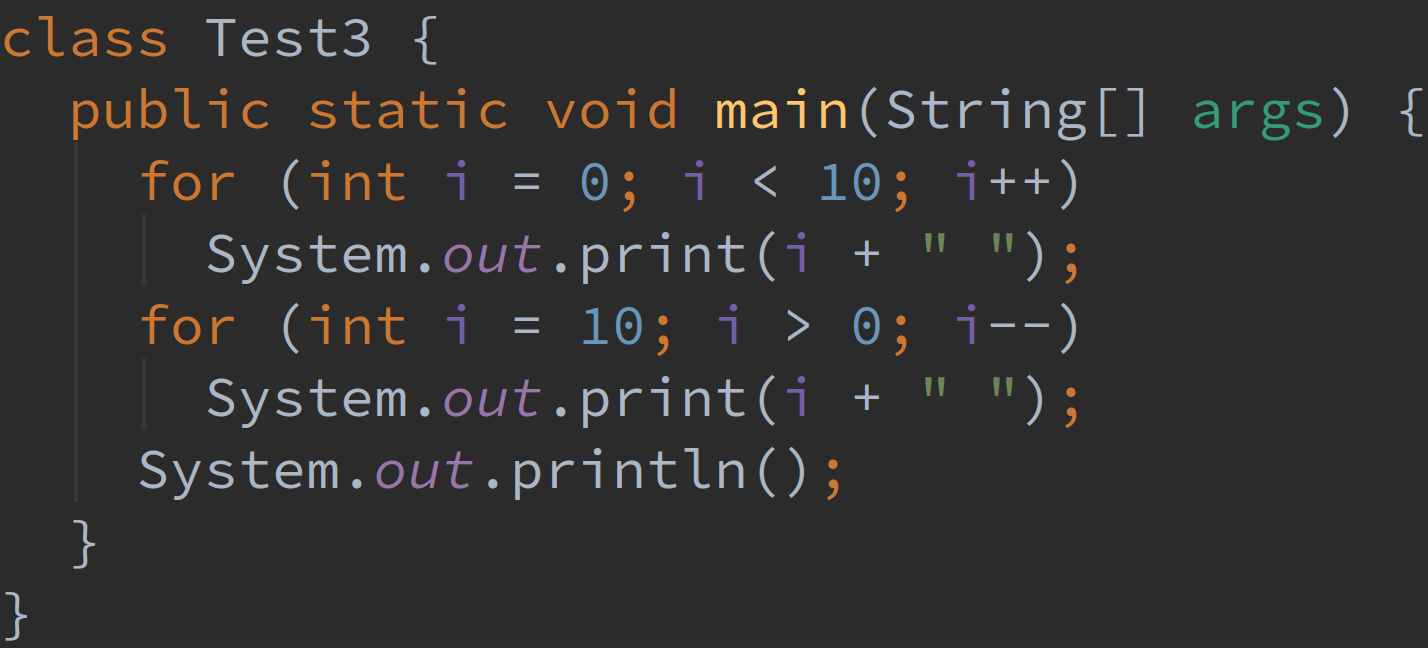
\includegraphics[width=\textwidth]{src/img/no-shadow.png}
        \caption{Two non-overlapping scopes \label{img:no-shadow}}
    \end{minipage}
\end{figure}

In the second example, it also means that the storage for the first \code{i} variable can be reused as the storage for
the second \code{i} variable, thus reducing the number of fields in the generated frame class, as at any moment during
the execution of the method, only one variable (formal parameter or local variable) of a certain name is in scope,
meaning that its value can be used in the code.

There are still problems if there is another variable in the method which shares the same name with other variable, but
whose type is different. If this other variable is not renamed, when generating the frame class, a compile-time error
will occur because JLS specifies that\footnote{\url{https://docs.oracle.com/javase/specs/jls/se8/html/jls-8.html#jls-FieldDeclaration}}:
\begin{quote}
    It is a compile-time error for the body of a class declaration to declare two fields with the same name.
\end{quote}

So all the relevant variables in the method (formal parameters and local variables) will be collected as fields of a
static nested frame class, which will be used by the recursive method to save the state of the method call when
recursing, thus simulating the call stack. The rule is that for all the variables with the same name and type, there
will be only one corresponding field in the frame class, but if there are variables with the same name, but different
type, each variable in a type group will have a different name and a different corresponding frame class field.

In other words, the first pass ensures that all the variables in a method which have the same name also have the same
type.

%TODO: Add example of renaming.
\section{Replacing \code{foreach} loops with \code{for} loops}

In Java, the \code{for} statement\footnote{\url{https://docs.oracle.com/javase/specs/jls/se8/html/jls-14.html#jls-14.14}}
has two forms: the basic one and the enhanced one. Since the meaning of the enhanced \code{for} statement is given by
translation into a basic \code{for} statement\footnote{\url{https://docs.oracle.com/javase/specs/jls/se8/html/jls-14.html#jls-14.14.2}},
the enhanced form is merely syntactic sugar for the basic one.

This pass first collects all the enhanced \code{for} statements in the method body which contain at least one recursive
call in pre-order fashion by using a visitor processing children nodes before the current node. Then it replaces these
statements by their equivalent basic \code{for} statements. This conversion is necessary because control flow needs to
be explicit for later stages in the refactoring process. The \textit{Condition} and \textit{Update} part of a \code{for}
statement in particular need to be explicit because they get executed after returning from a recursive call in the body
of the \code{for} statement.

There are two cases for this conversion: the first when the type of \textit{Expression} is a subtype of
\texttt{Iterable} (exemplified in \labelindexref{Figure}{img:foreach-to-iterator-for-before} and
\labelindexref{Figure}{img:foreach-to-iterator-for-after}) and the second when \textit{Expression} has an array type
\texttt{T[]} (exemplified in \labelindexref{Figure}{img:foreach-to-indexed-for-before} and
\labelindexref{Figure}{img:foreach-to-indexed-for-after}), where \textit{Expression} is the value over which the
enhanced \code{for} statement iterates.

\fig[height=0.5in]{src/img/foreach-to-iterator-for-before.png}{img:foreach-to-iterator-for-before}{\code{Foreach} loop to iterator \code{for} loop conversion (before)}
\fig[height=0.625in]{src/img/foreach-to-iterator-for-after.png}{img:foreach-to-iterator-for-after}{\code{Foreach} loop to iterator \code{for} loop conversion (after)}
%\fig[width=.3\textwidth]{src/img/foreach-to-indexed-for-before.png}{img:foreach-to-indexed-for-before}{\code{Foreach} loop to indexed \code{for} loop conversion (before)}
%\fig[width=.4\textwidth]{src/img/foreach-to-indexed-for-after.png}{img:foreach-to-indexed-for-after}{\code{Foreach} loop to indexed \code{for} loop conversion (before)}
\begin{figure}[!tbp]
    \centering
    \begin{minipage}[b]{0.45\textwidth}
        \begin{center}
            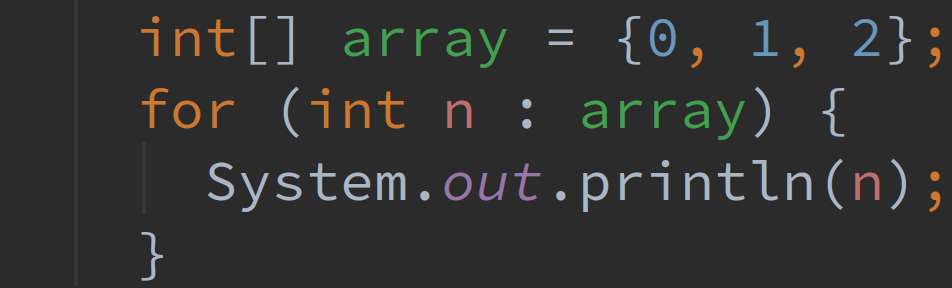
\includegraphics[height=0.5in]{src/img/foreach-to-indexed-for-before.png}
            \caption{\code{Foreach} loop to indexed \code{for} loop conversion (before) \label{img:foreach-to-indexed-for-before}}
        \end{center}
    \end{minipage}
    \hfill
    \begin{minipage}[b]{0.45\textwidth}
        \begin{center}
            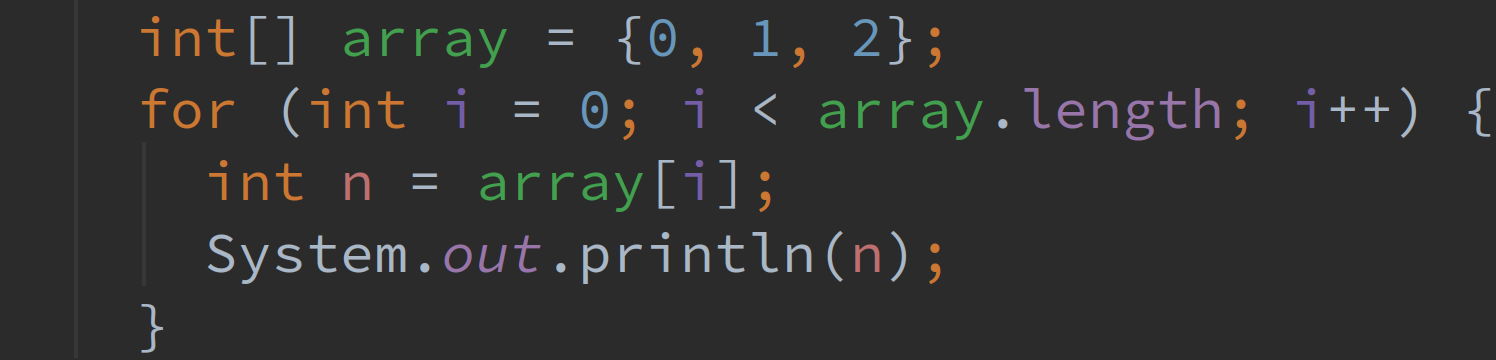
\includegraphics[height=0.625in]{src/img/foreach-to-indexed-for-after.png}
            \caption{\code{Foreach} loop to indexed \code{for} loop conversion (before) \label{img:foreach-to-indexed-for-after}}
        \end{center}
    \end{minipage}
\end{figure}
%These two conversions are carried out using the ones that Intellij IDEA provides as intentions.
\section{Replacing single statements with block statements}

Given the fact that Java allows some statements to appear outside of a block, they may cause problems in later steps of
the algorithm when processing the statements of a block. For example, if a new statement needs to be added before or
after another statement which is not part of a block, the initial statement needs to be first enclosed in a block, in
which the other statement will be added at the right place.
The places where this pass is applied are the branches of
\code{if}\footnote{\url{https://docs.oracle.com/javase/specs/jls/se8/html/jls-14.html#jls-14.9}} statements and the
bodies of \code{for}\footnote{\url{https://docs.oracle.com/javase/specs/jls/se8/html/jls-14.html#jls-14.14.1}},
\code{foreach}\footnote{\url{https://docs.oracle.com/javase/specs/jls/se8/html/jls-14.html#jls-14.14.2}},
\code{while}\footnote{\url{https://docs.oracle.com/javase/specs/jls/se8/html/jls-14.html#jls-14.12}} and
\code{do-while}\footnote{\url{https://docs.oracle.com/javase/specs/jls/se8/html/jls-14.html#jls-14.13}} statements
which contain single statements. If the single statement is an instance of
\code{PsiEmptyStatement}\footnote{\url{https://docs.oracle.com/javase/specs/jls/se8/html/jls-14.html#jls-14.6}},
it gets replaced with an empty block instead of a block containing an empty statement, because this would be redundant.

A special case is the \code{switch}\footnote{\url{https://docs.oracle.com/javase/specs/jls/se8/html/jls-14.html#jls-14.11}}
statement. The pass replaces the statements after each \code{switch} label (both \code{case} and \code{default} labels)
up to the next \code{switch} label (no next one when the label is the last) with a block containing these statements.
This transformation does not alter the semantics of the \code{switch} statement.

This pass also transforms statements which may not contain recursive calls, because there are elements which the
refactoring alters in order to remove recursion and they are not only method calls (for example, \code{return}
statements). An example is provided in \labelindexref{Figure}{img:replace-single-statements-with-block-statements}.

\begin{figure}[htb]
    \makebox[\linewidth][c]{%
    \begin{subfigure}[b]{.6\textwidth}
        \centering
        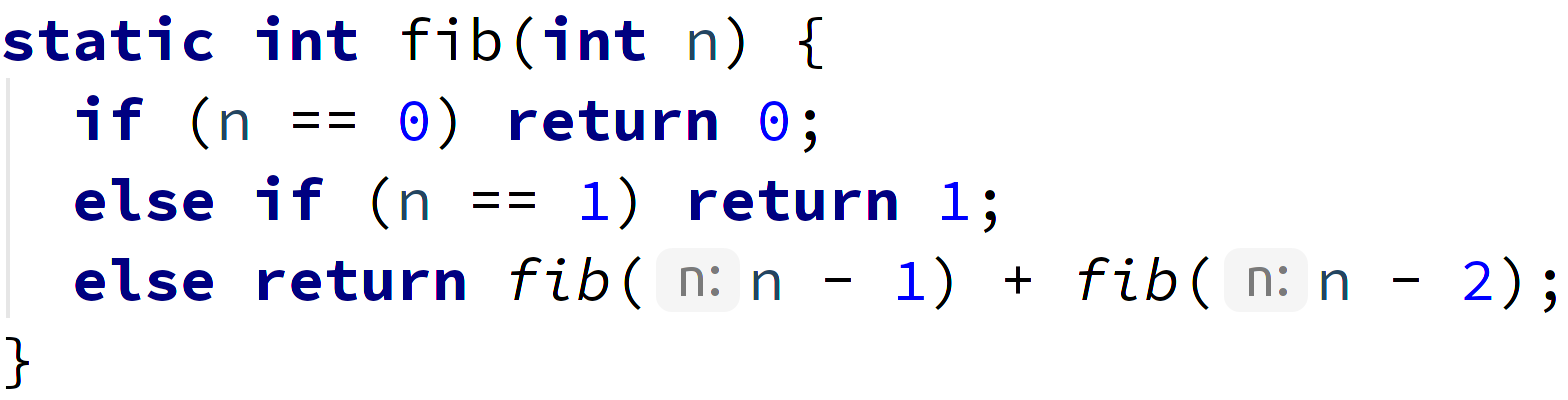
\includegraphics[height=0.6in]{src/img/replace-single-statements-with-block-statements-before-white.png}
        \caption{Before}
    \end{subfigure}%
    \begin{subfigure}[b]{.6\textwidth}
        \centering
        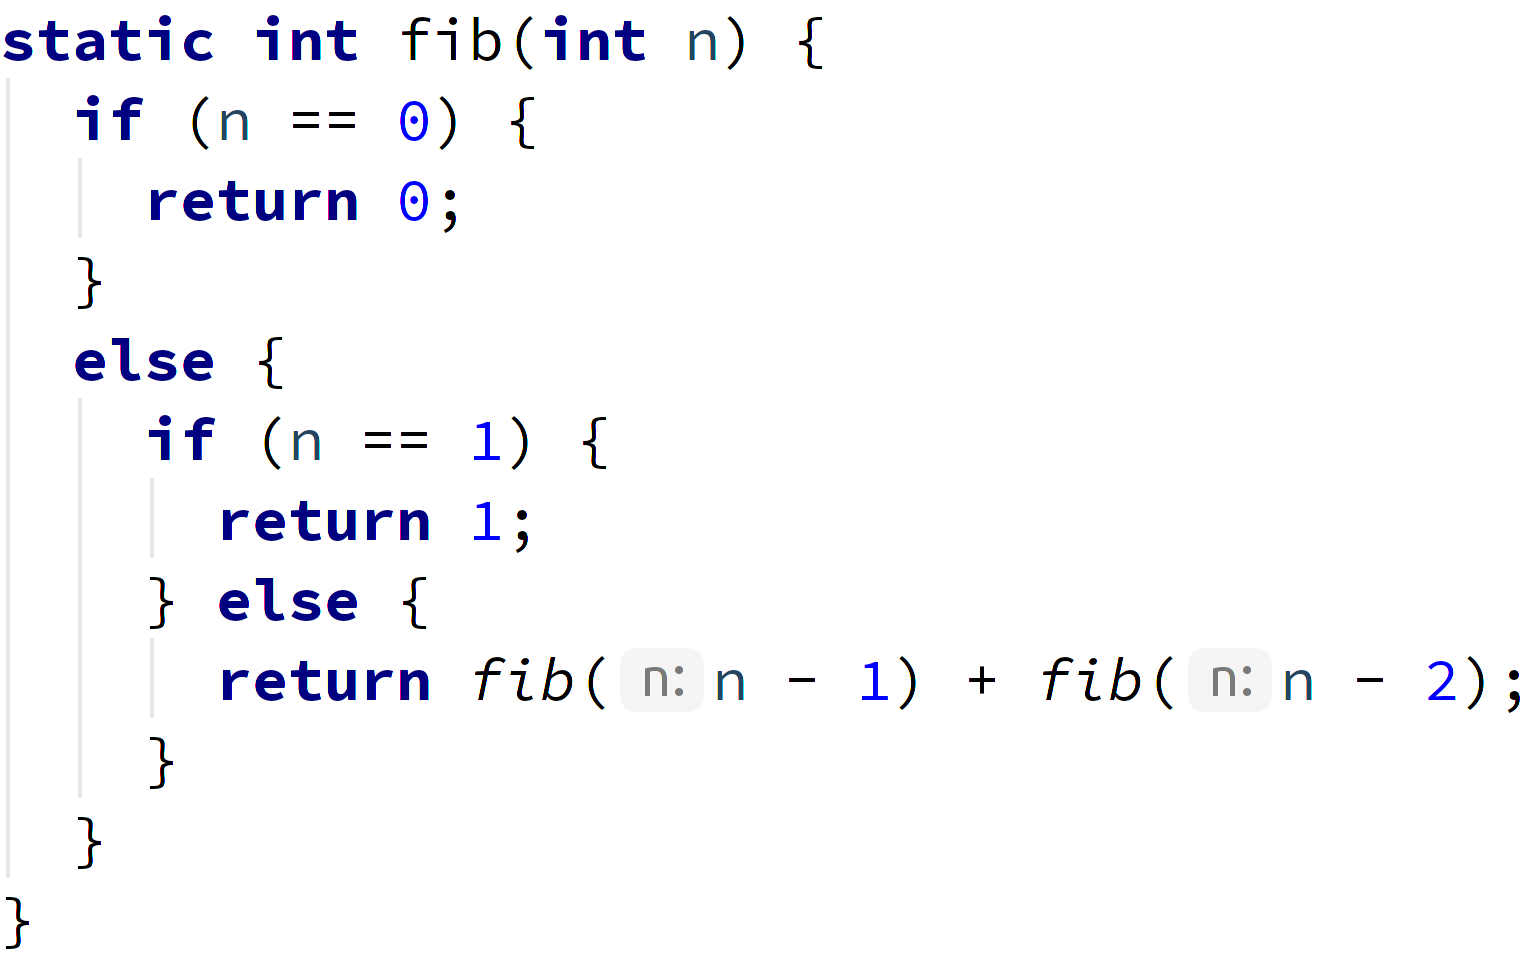
\includegraphics[height=1.44in]{src/img/replace-single-statements-with-block-statements-after-white.png}
        \caption{After}
    \end{subfigure}%
    }\\
    \caption{Replacing single statements with block statements \label{img:replace-single-statements-with-block-statements}}
\end{figure}
\section{Extracting recursive calls to statements}

This pass extracts recursive calls in the method body to separate statements
(\textit{LocalVariableDeclarationStatement}s\footnote{\url{https://docs.oracle.com/javase/specs/jls/se8/html/jls-14.html#jls-LocalVariableDeclarationStatement}}
with the method call as the
\textit{VariableInitializer}\footnote{\url{https://docs.oracle.com/javase/specs/jls/se8/html/jls-8.html#jls-VariableInitializer}}),
if the call is not already the \textit{VariableInitializer} of a \textit{LocalVariableDeclarationStatement} or the
right-hand side of an \textit{Assignment}\footnote{\url{https://docs.oracle.com/javase/specs/jls/se8/html/jls-15.html#jls-Assignment}}
having an \textit{ExpressionStatement}\footnote{\url{https://docs.oracle.com/javase/specs/jls/se8/html/jls-14.html#jls-ExpressionStatement}}
as parent. The pass does not affect recursive methods with \code{void} return type, because recursive calls to these
methods are already part of a separate \textit{ExpressionStatement}.

This code modification is necessary because the expression in which a recursive call may be embedded gets evaluated
only after returning from the recursive call. By separating the point of return from recursion from the following
computations, it will be possible to jump in the method body to the statements after the call.
\section{Adding the frame class}

Some of the previous passes potentially add new local variables to the method. \textit{Renaming variables to unique
names} adds new variables by renaming the ones which could generate name clashes in this pass.
\textit{Replacing \code{foreach} loops with \code{for} loops} adds a new \code{iterator} variable for iterator-based
\code{foreach} loops and an index variable \code{i} for array-based \code{foreach} loops. If there is already a local
variable named \code{iterator} or \code{i}, in the method body, the pass generates a unique variable name by appending
indexes to these names, to avoid name clashes. The third pass which may add new local variables is
\textit{Extracting recursive calls to statements}, because the recursive calls are extracted to local variable
declaration statements named \code{temp}, with potential name clashes being again avoided with indexes, if necessary.

This pass generates a \code{private static} nested class named by the capitalized name of the method followed by the
\code{Frame} suffix. The fields of the frame class represent the variables of the method (both formal parameters and
local variables) which are relevant after a recursive call (whose scope contains at least a recursive call). They are
declared as \code{private}, because the enclosing class can still access the fields of this class. The frame class also
contains a \code{private} constructor which initializes only the fields representing the formal parameters of the
method, because the fields corresponding to local variables are initialized by assignment in the method body,
after another pass. Until they are initialized in the method body, they have the corresponding default values.
By virtue of \textit{Definite Assignment}\footnote{\url{https://docs.oracle.com/javase/specs/jls/se8/html/jls-16.html}},
provided that the method compiles without errors before the refactoring, there will not be any problems involving using
uninitialized local variables.

There is an additional \code{int} field named \code{block} in the frame class, which represents the index of the
block of code to which the method jumps when returning from the callee to continue executing the statements in the
caller after the recursive call.

An example of a frame class in provided in \labelindexref{Figure}{img:add-frame-class}.
The frame class contains the formal parameters of the method as fields. The field \code{iterator} has been generated
because the \code{foreach} loop has been converted to a \code{for} loop, since it contains a recursive call. The
variable \code{n} is added as a corresponding field to the frame class, because its scope contains a recursive call.
On the other hand, the local variable \code{ctc} does not have a corresponding field in the frame class, because its
scope does not include a recursive call. Finally, the \code{block} field is added to the fields of the frame class.

\begin{figure}[htb]
    \makebox[\linewidth][c]{%
    \begin{subfigure}[b]{.5\textwidth}
        \centering
        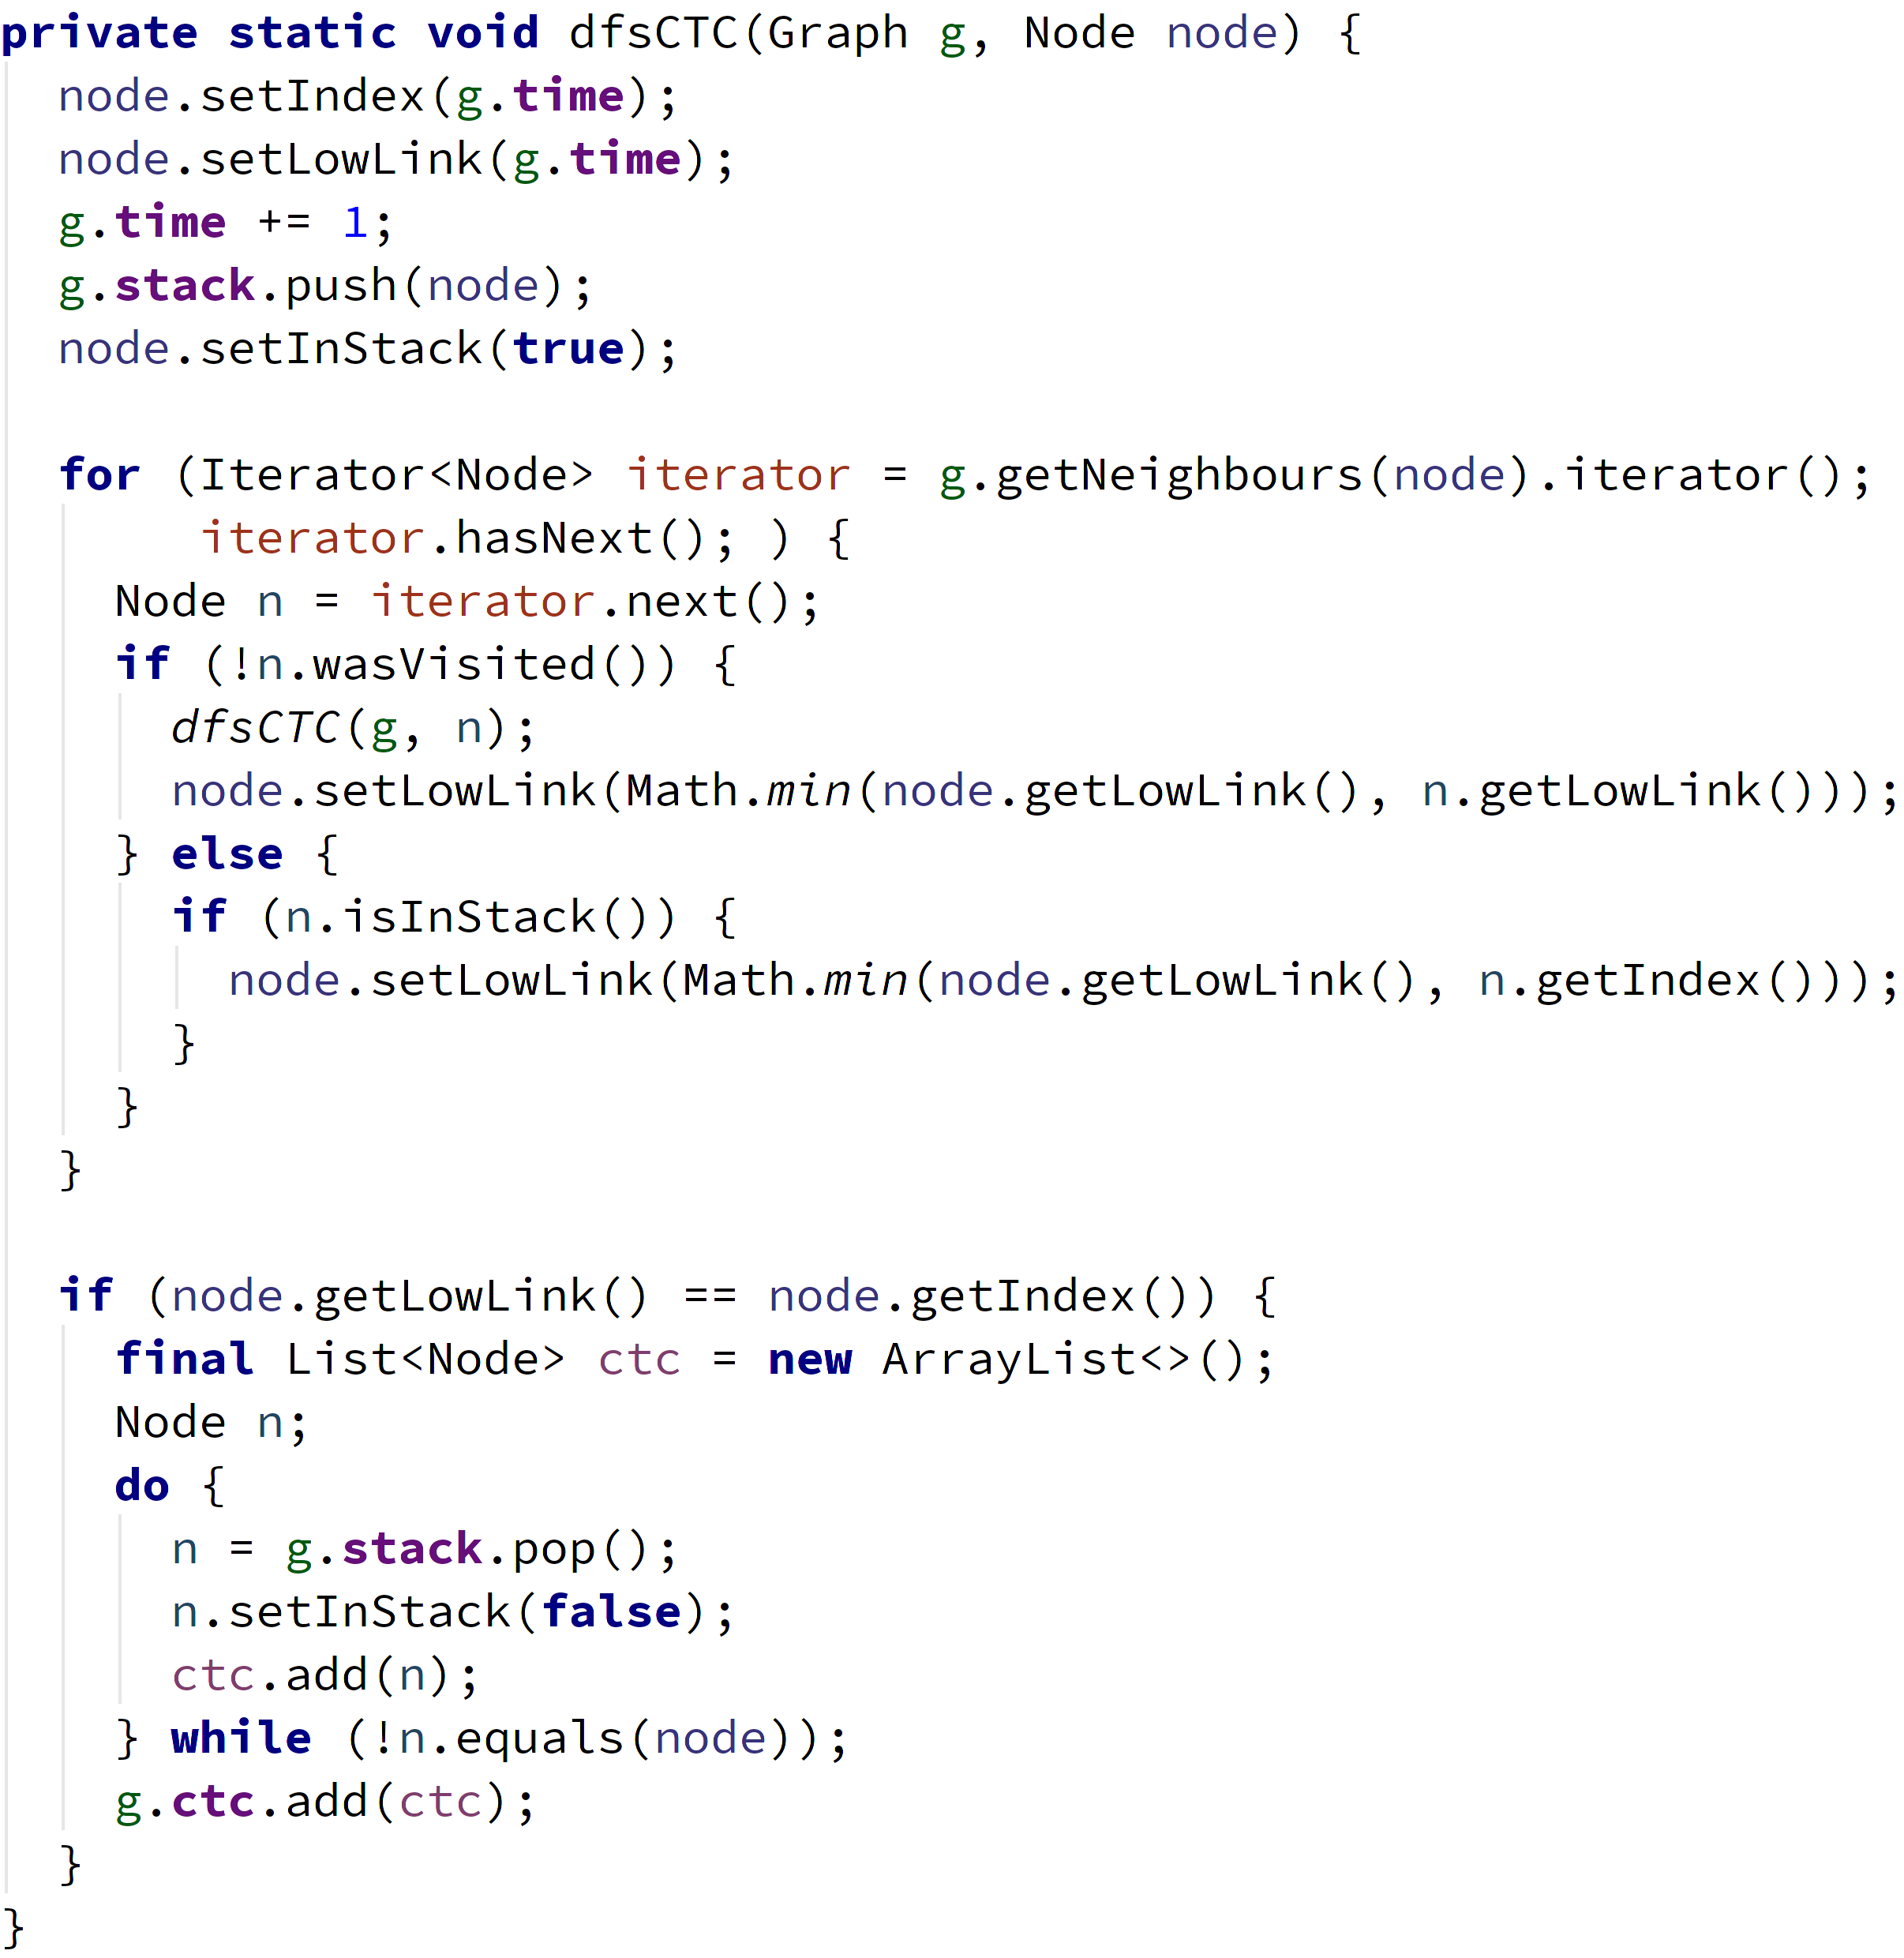
\includegraphics[height=2.5in]{src/img/add-frame-class-before-white-31.png}
        \caption{Before}
    \end{subfigure}%
    \begin{subfigure}[b]{.5\textwidth}
        \centering
        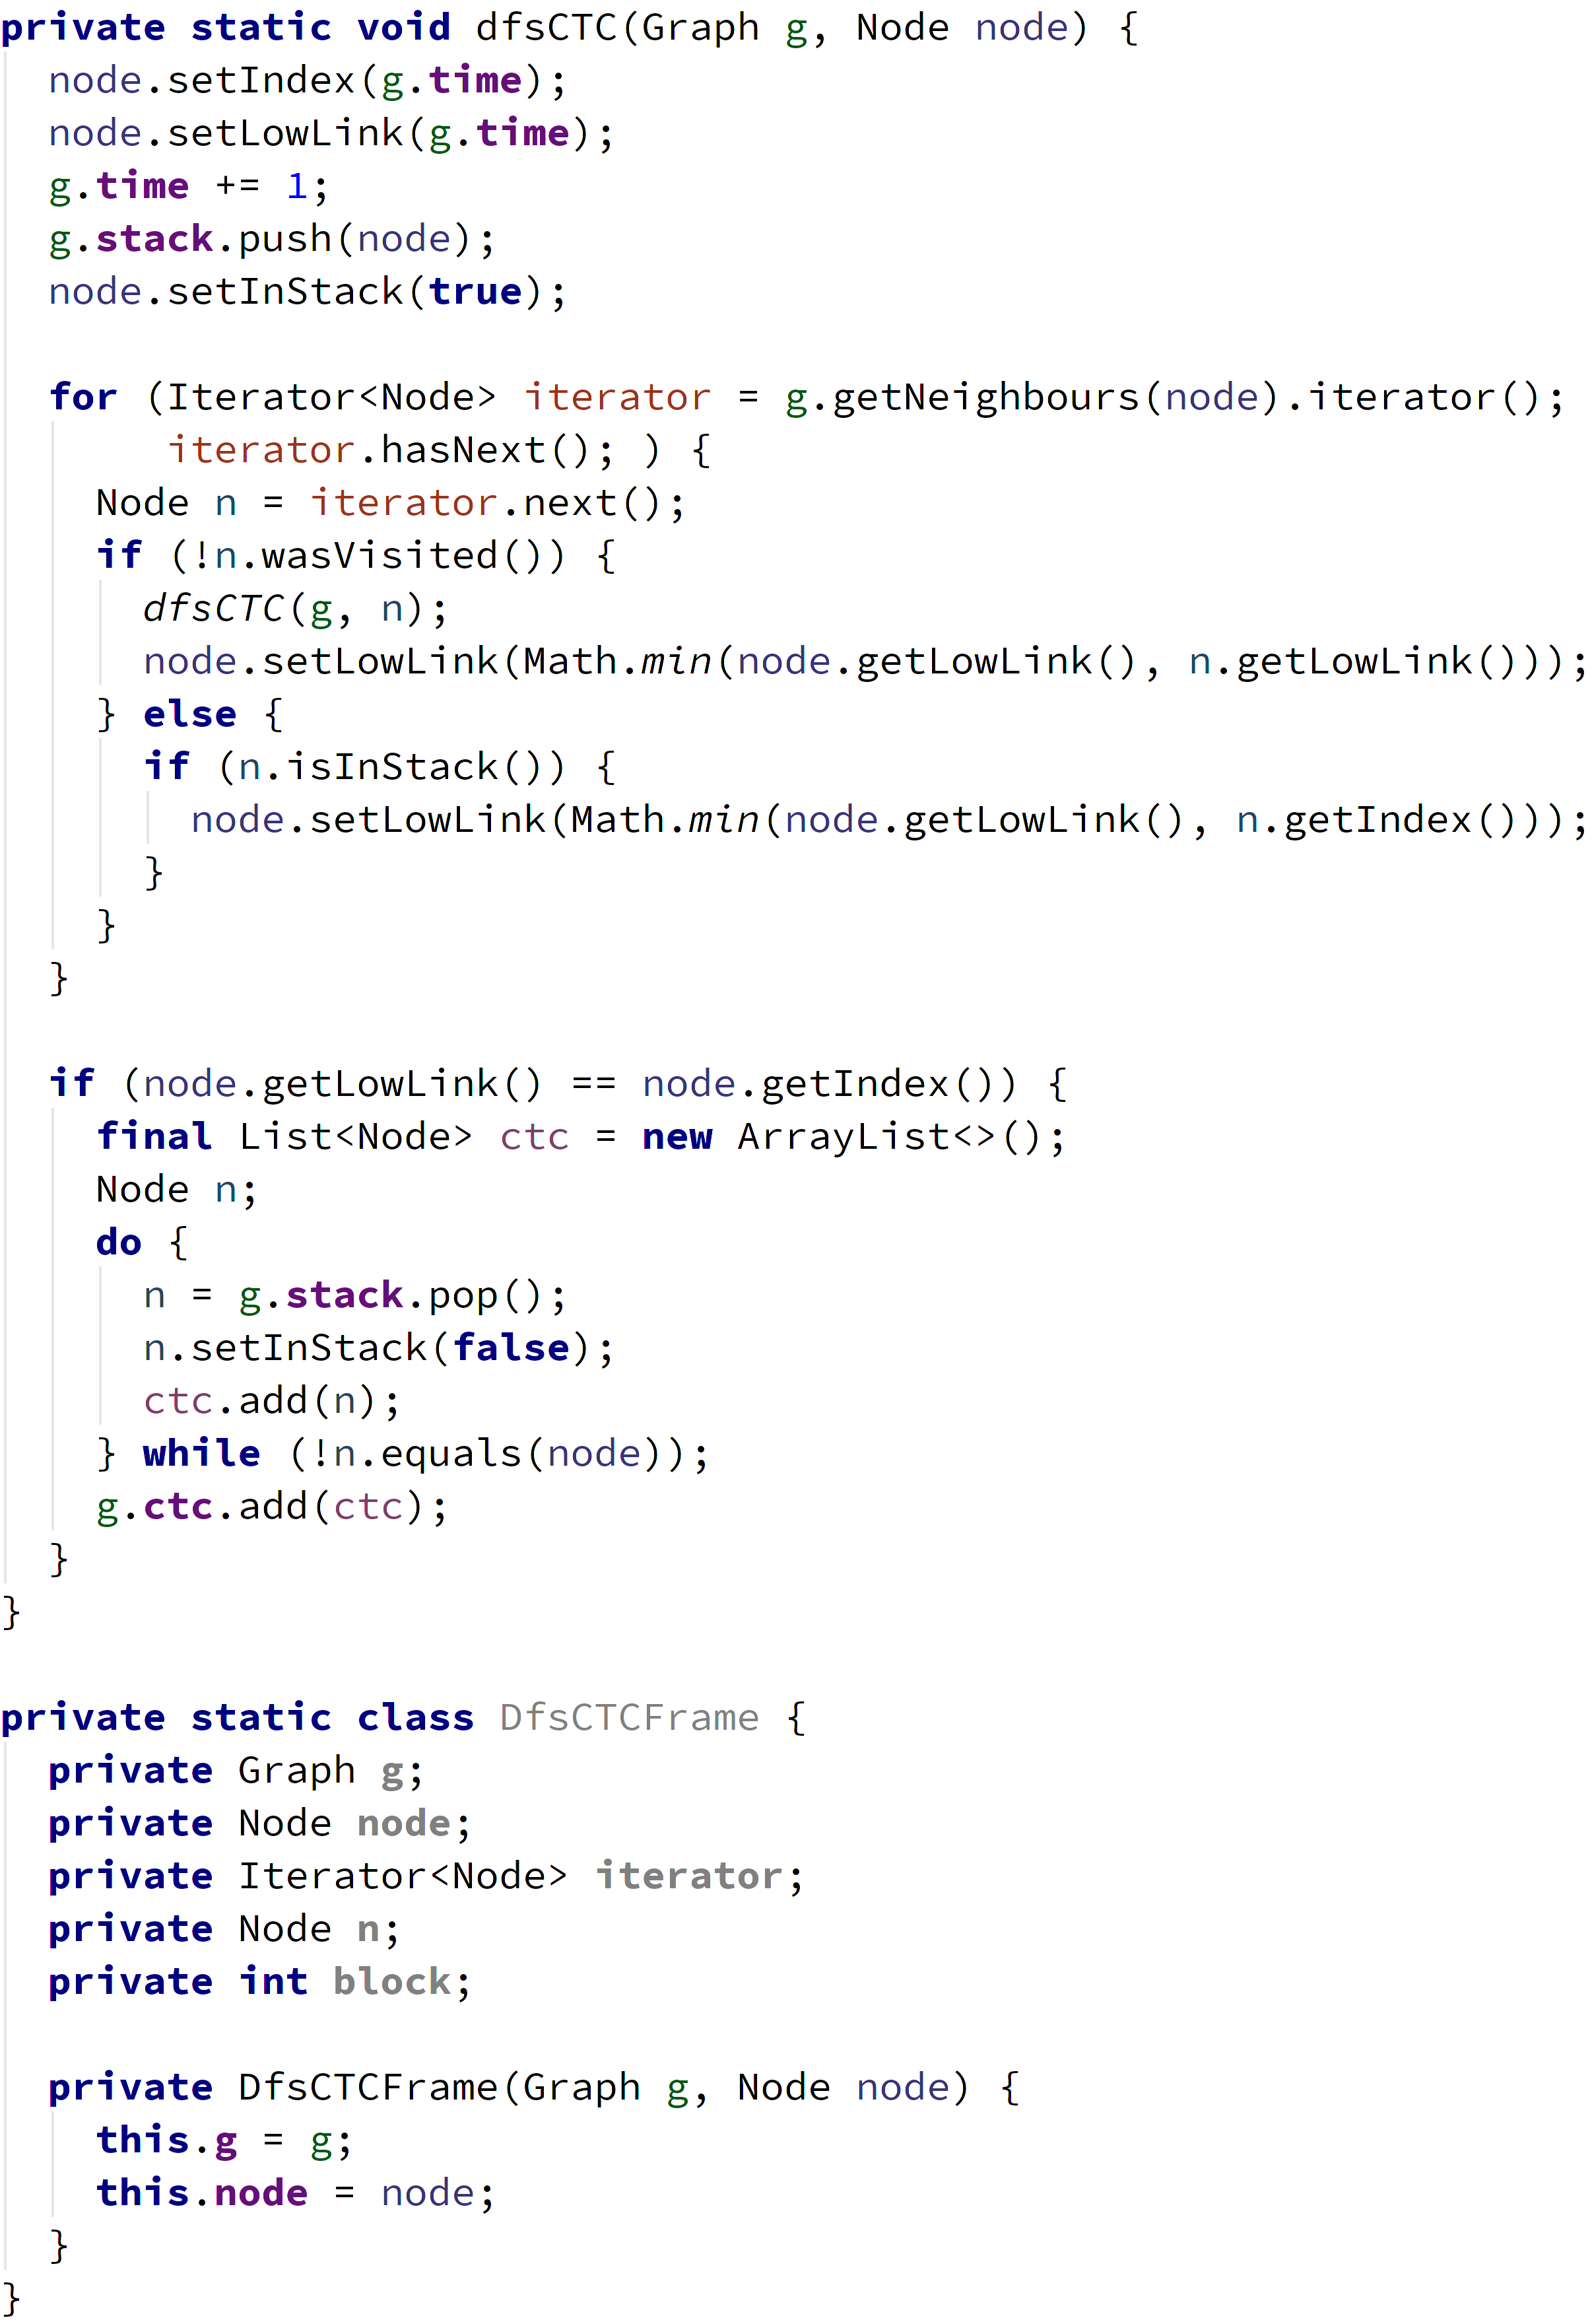
\includegraphics[height=3.548in]{src/img/add-frame-class-after-white-44.png}
        \caption{After}
    \end{subfigure}%
    }\\
    \caption{Adding the frame class \label{img:add-frame-class}}
\end{figure}
\section{Incorporating the body}

The passes so far have been preparatory ones, such that the main part of the algorithm can take place without problems.
This pass may seem out of place, but its purpose is to ensure that each code manipulation until the final result still
produces valid code, because this requirement is necessary later for resolving the method calls to the called methods
and finding the usages of the local variables using the infrastructure provided by Intellij IDEA.

The call stack will be simulated in the method body by using a \code{stack} object. Whenever there is a call to the
containing method, a new frame object will be pushed onto the \code{stack}. This is why after declaring the \code{stack}
object, the next statement in the body of the method is a \code{push} call, with the arguments equal to the formal
parameters. This frame represents the first method call from outside this method.

If the return type of the method is not \code{void}, the next statement in the method body will be a declaration
statement of a local variable named \code{ret}, which will be used to save the return value of the callee, to be used
later by the caller of a recursive call.

The next statement is a \code{while} statement which loops as long as the simulated call \code{stack} is not empty.
Because the body of the statement will execute the code in the context of a current stack \code{frame},
the first statement in the \code{while} body is a declaration statement of a local variable named \code{frame},
initialized as the frame at the top of the call stack. After this statement, the original body of the method will be
included here as a block statement.

If the return type of the method is not \code{void}, there will be a final \code{return} statement in the method body
after the \code{while} statement, which will return the value of the \code{ret} local variable, which will hold the
return value of the method after the control flow exits the \code{while} statement.

An example of this pass is provided in \labelindexref{Figure}{img:incorporate}.

\begin{figure}[htb]
    \makebox[\linewidth][c]{%
    \begin{subfigure}[b]{.6\textwidth}
        \centering
        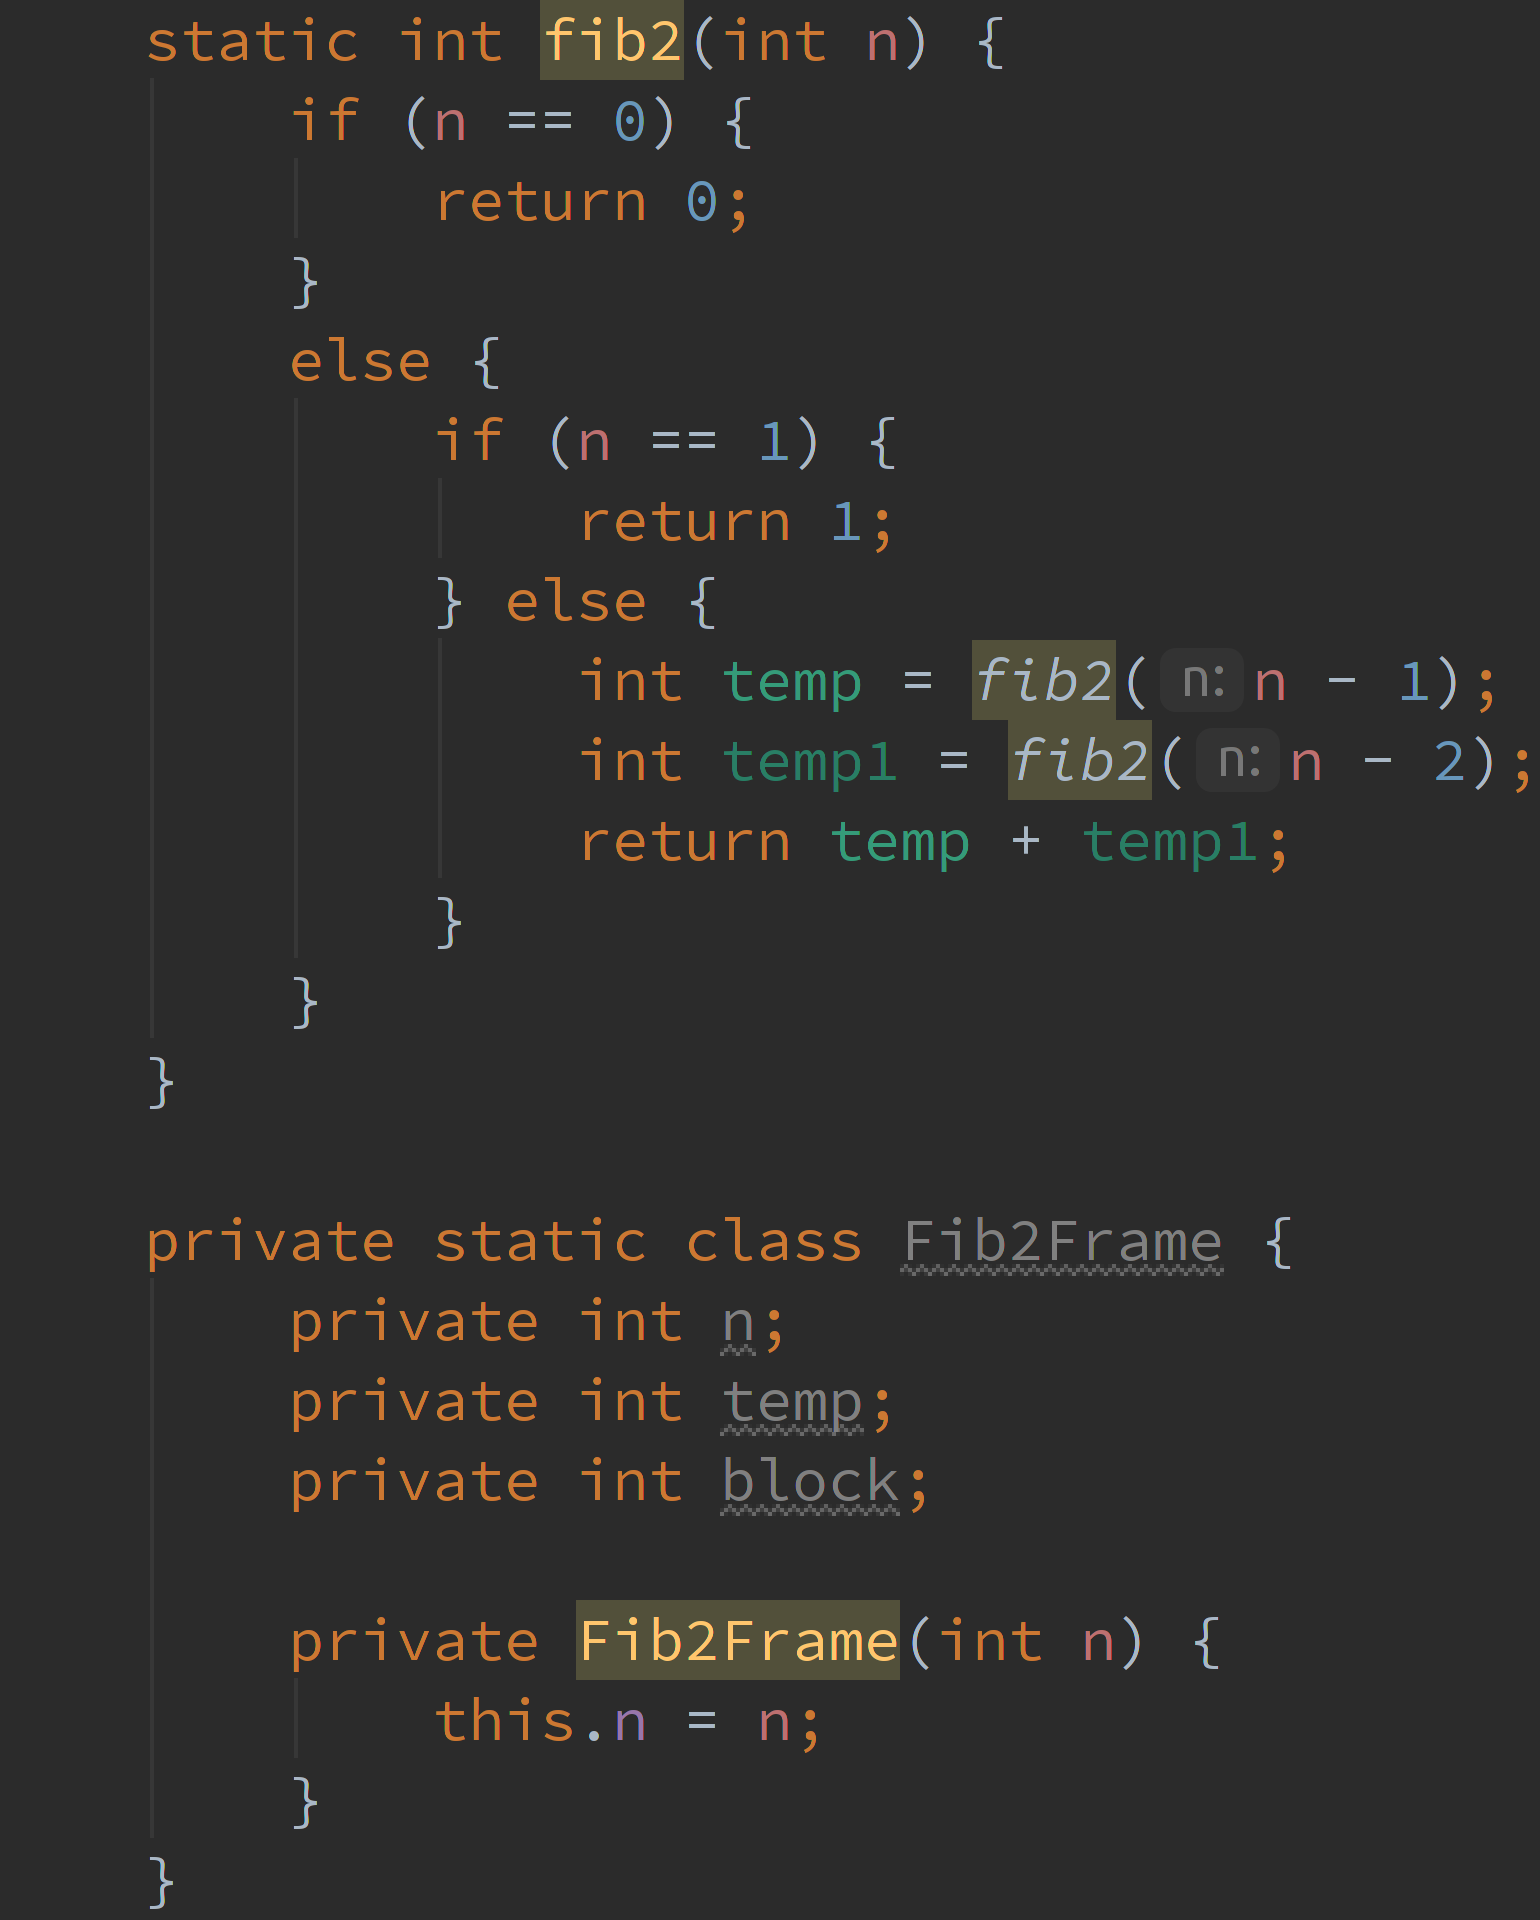
\includegraphics[height=2.5in]{src/img/incorporate-before.png}
        \caption{Before}
    \end{subfigure}%
    \begin{subfigure}[b]{.6\textwidth}
        \centering
        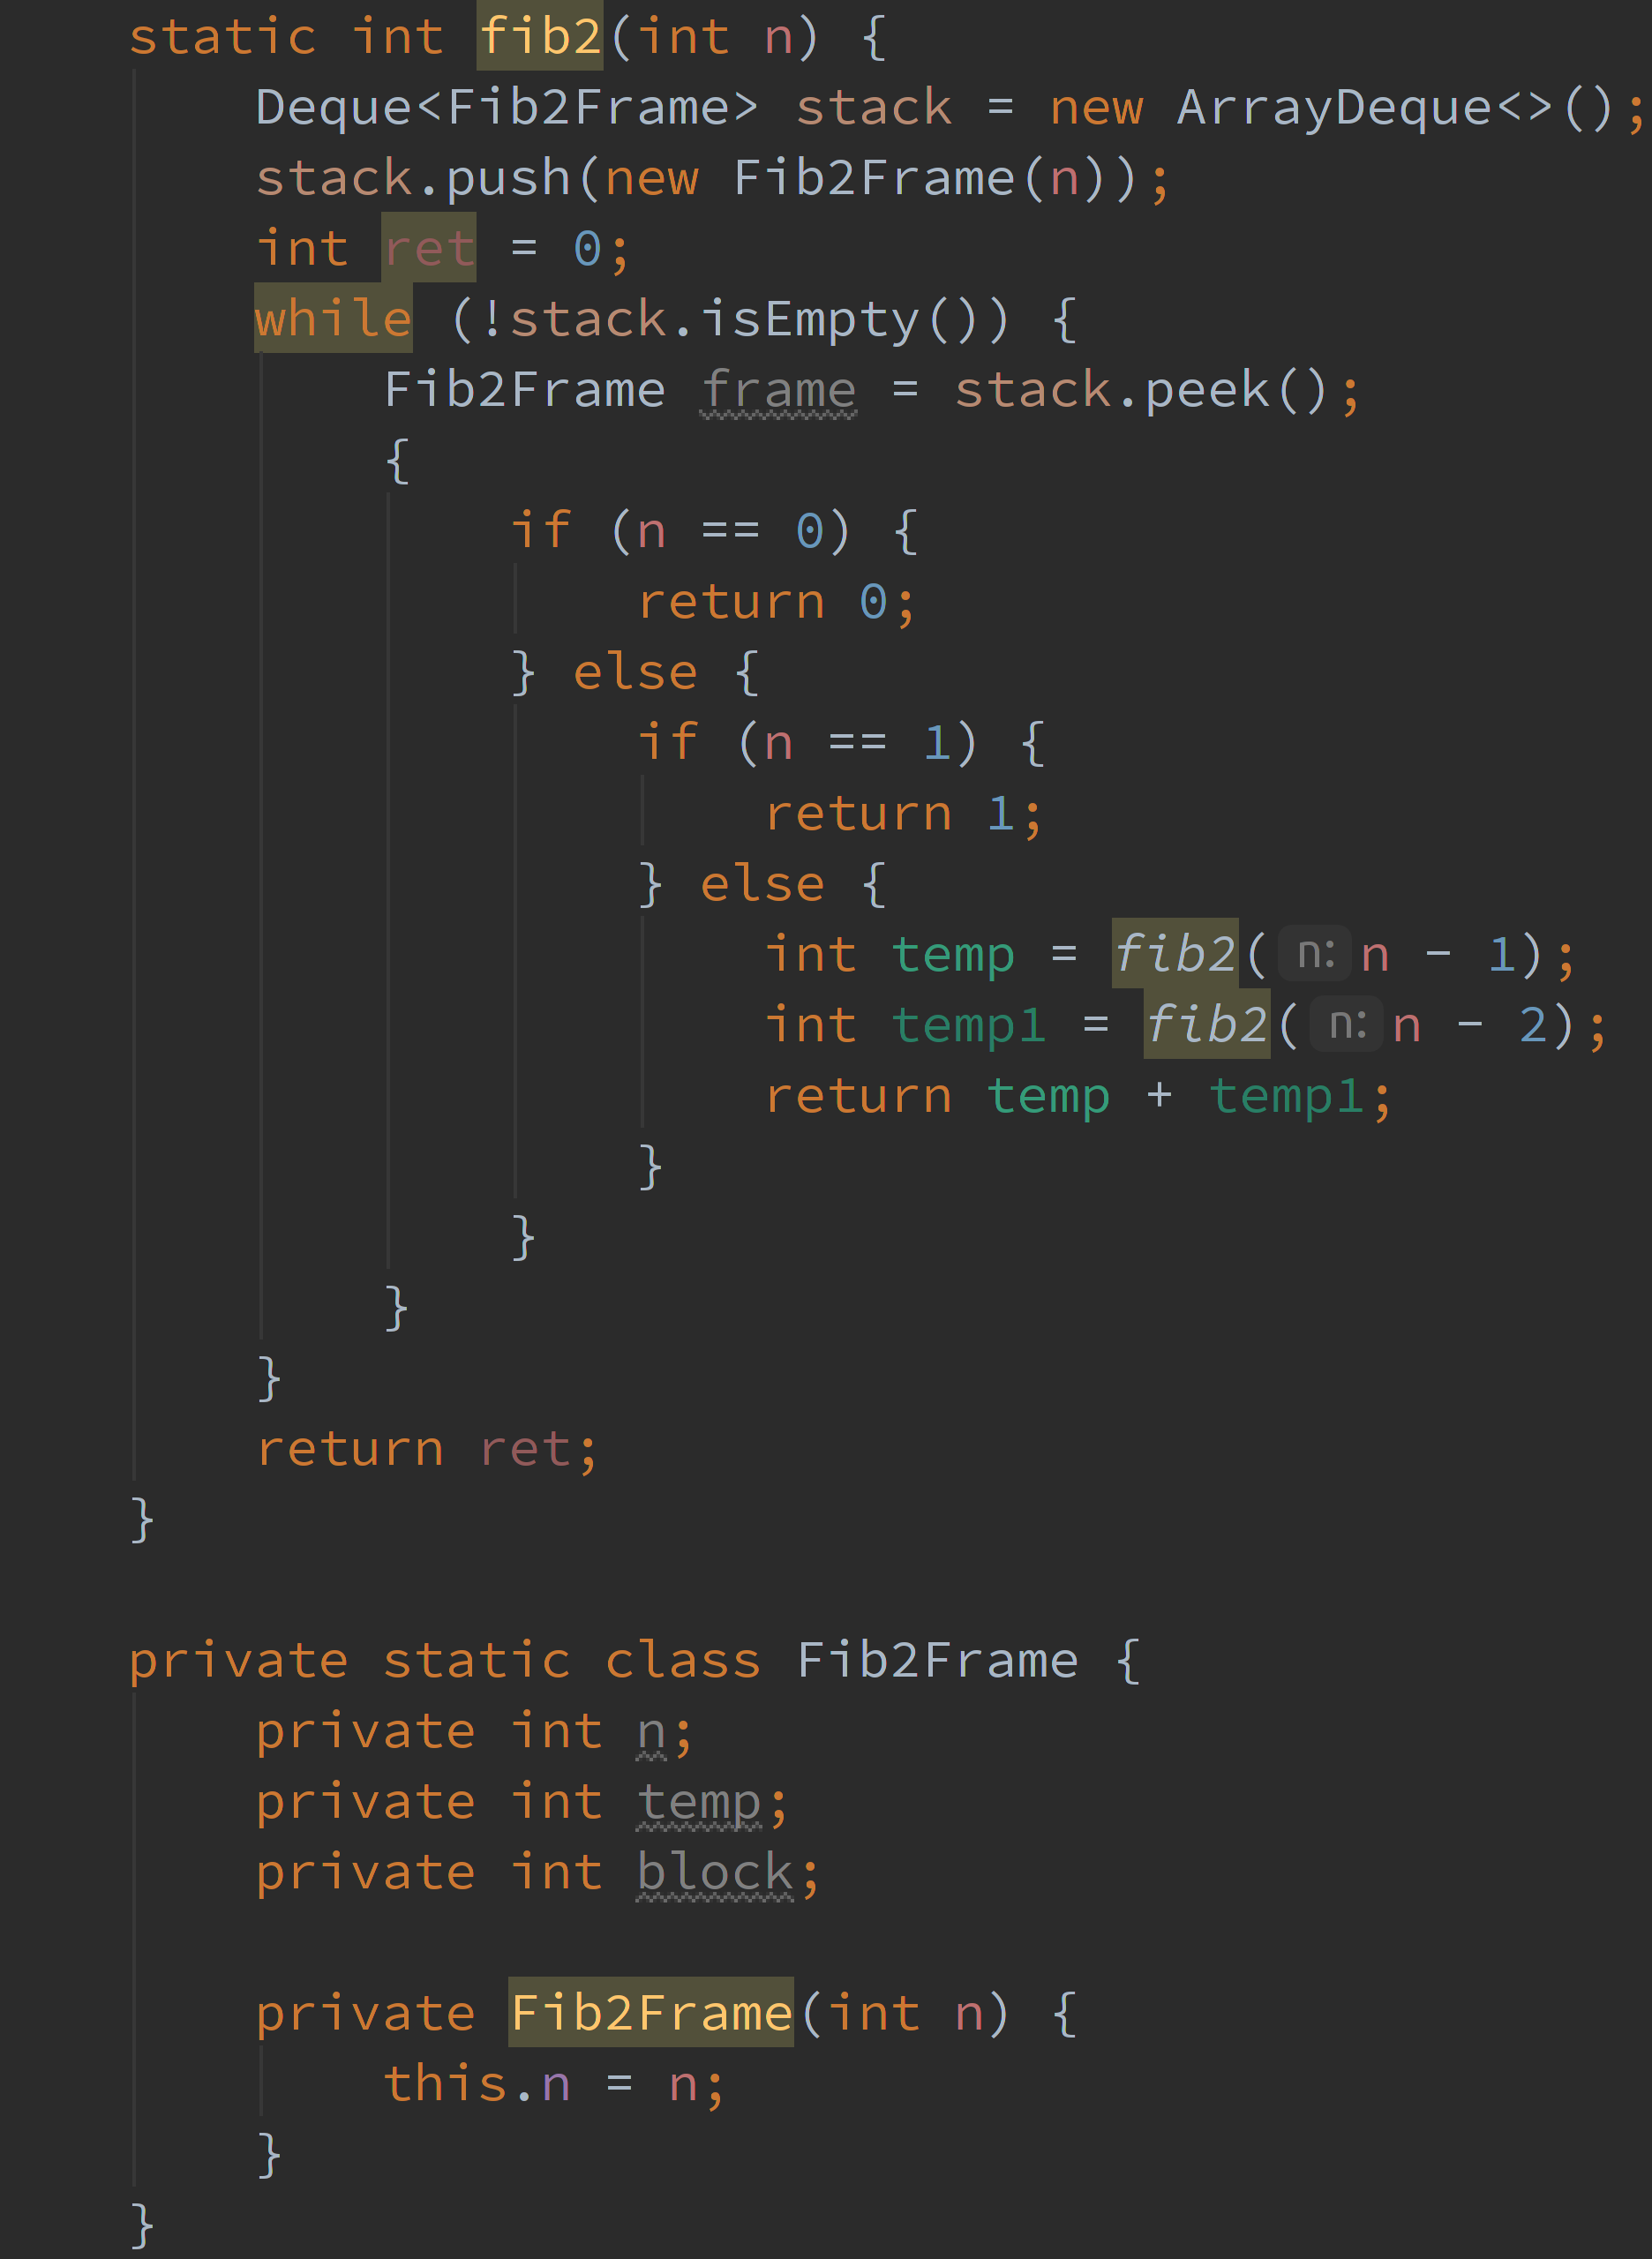
\includegraphics[height=3.33in]{src/img/incorporate-after.png}
        \caption{After}
    \end{subfigure}%
    }\\
    \caption{Incorporating the body \label{img:incorporate}}
\end{figure}
\section{Replacing references with frame accesses}

This pass replaces references to the relevant formal parameters and local variables in the original body of the method
with field accesses to the corresponding fields of the \code{frame} object, where relevant refers to variables whose
scope contains at least one recursive call.

An example of this pass is provided in \labelindexref{Figure}{img:replace-identifier}.

\begin{figure}[htb]
    \makebox[\linewidth][c]{%
    \begin{subfigure}[b]{.6\textwidth}
        \centering
        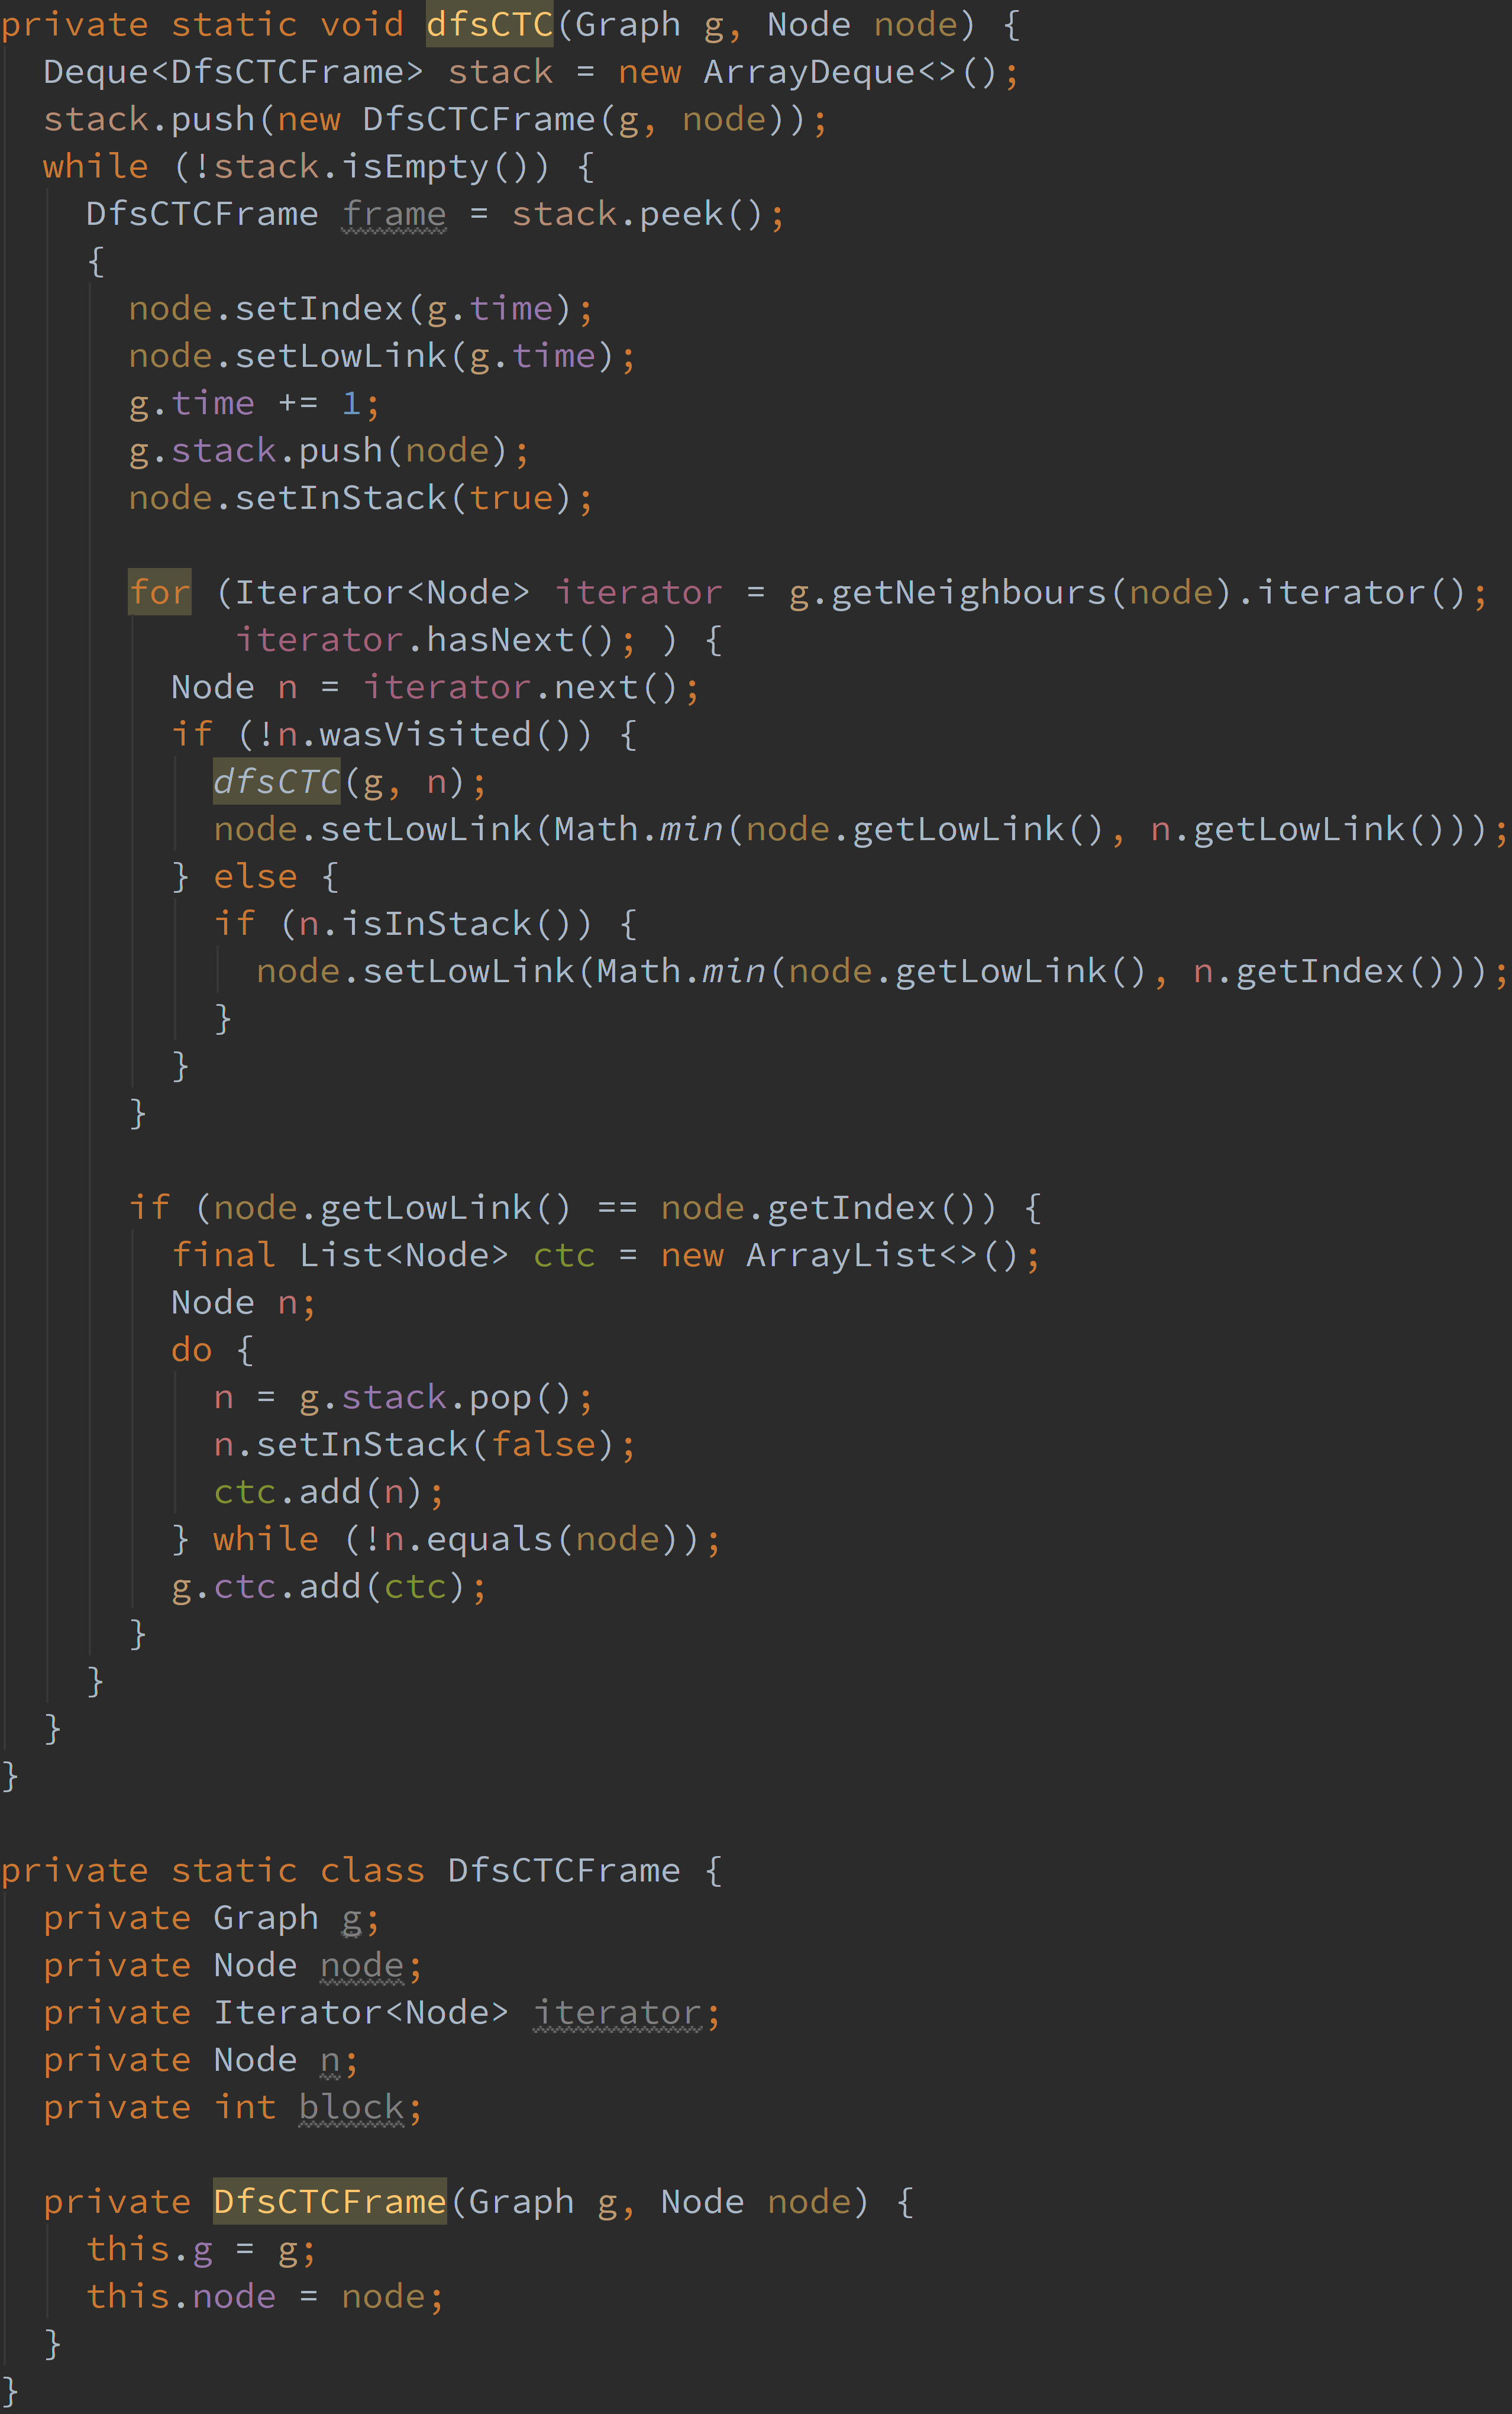
\includegraphics[height=3.7in]{src/img/replace-identifier-before.png}
        \caption{Before}
    \end{subfigure}%
    \begin{subfigure}[b]{.6\textwidth}
        \centering
        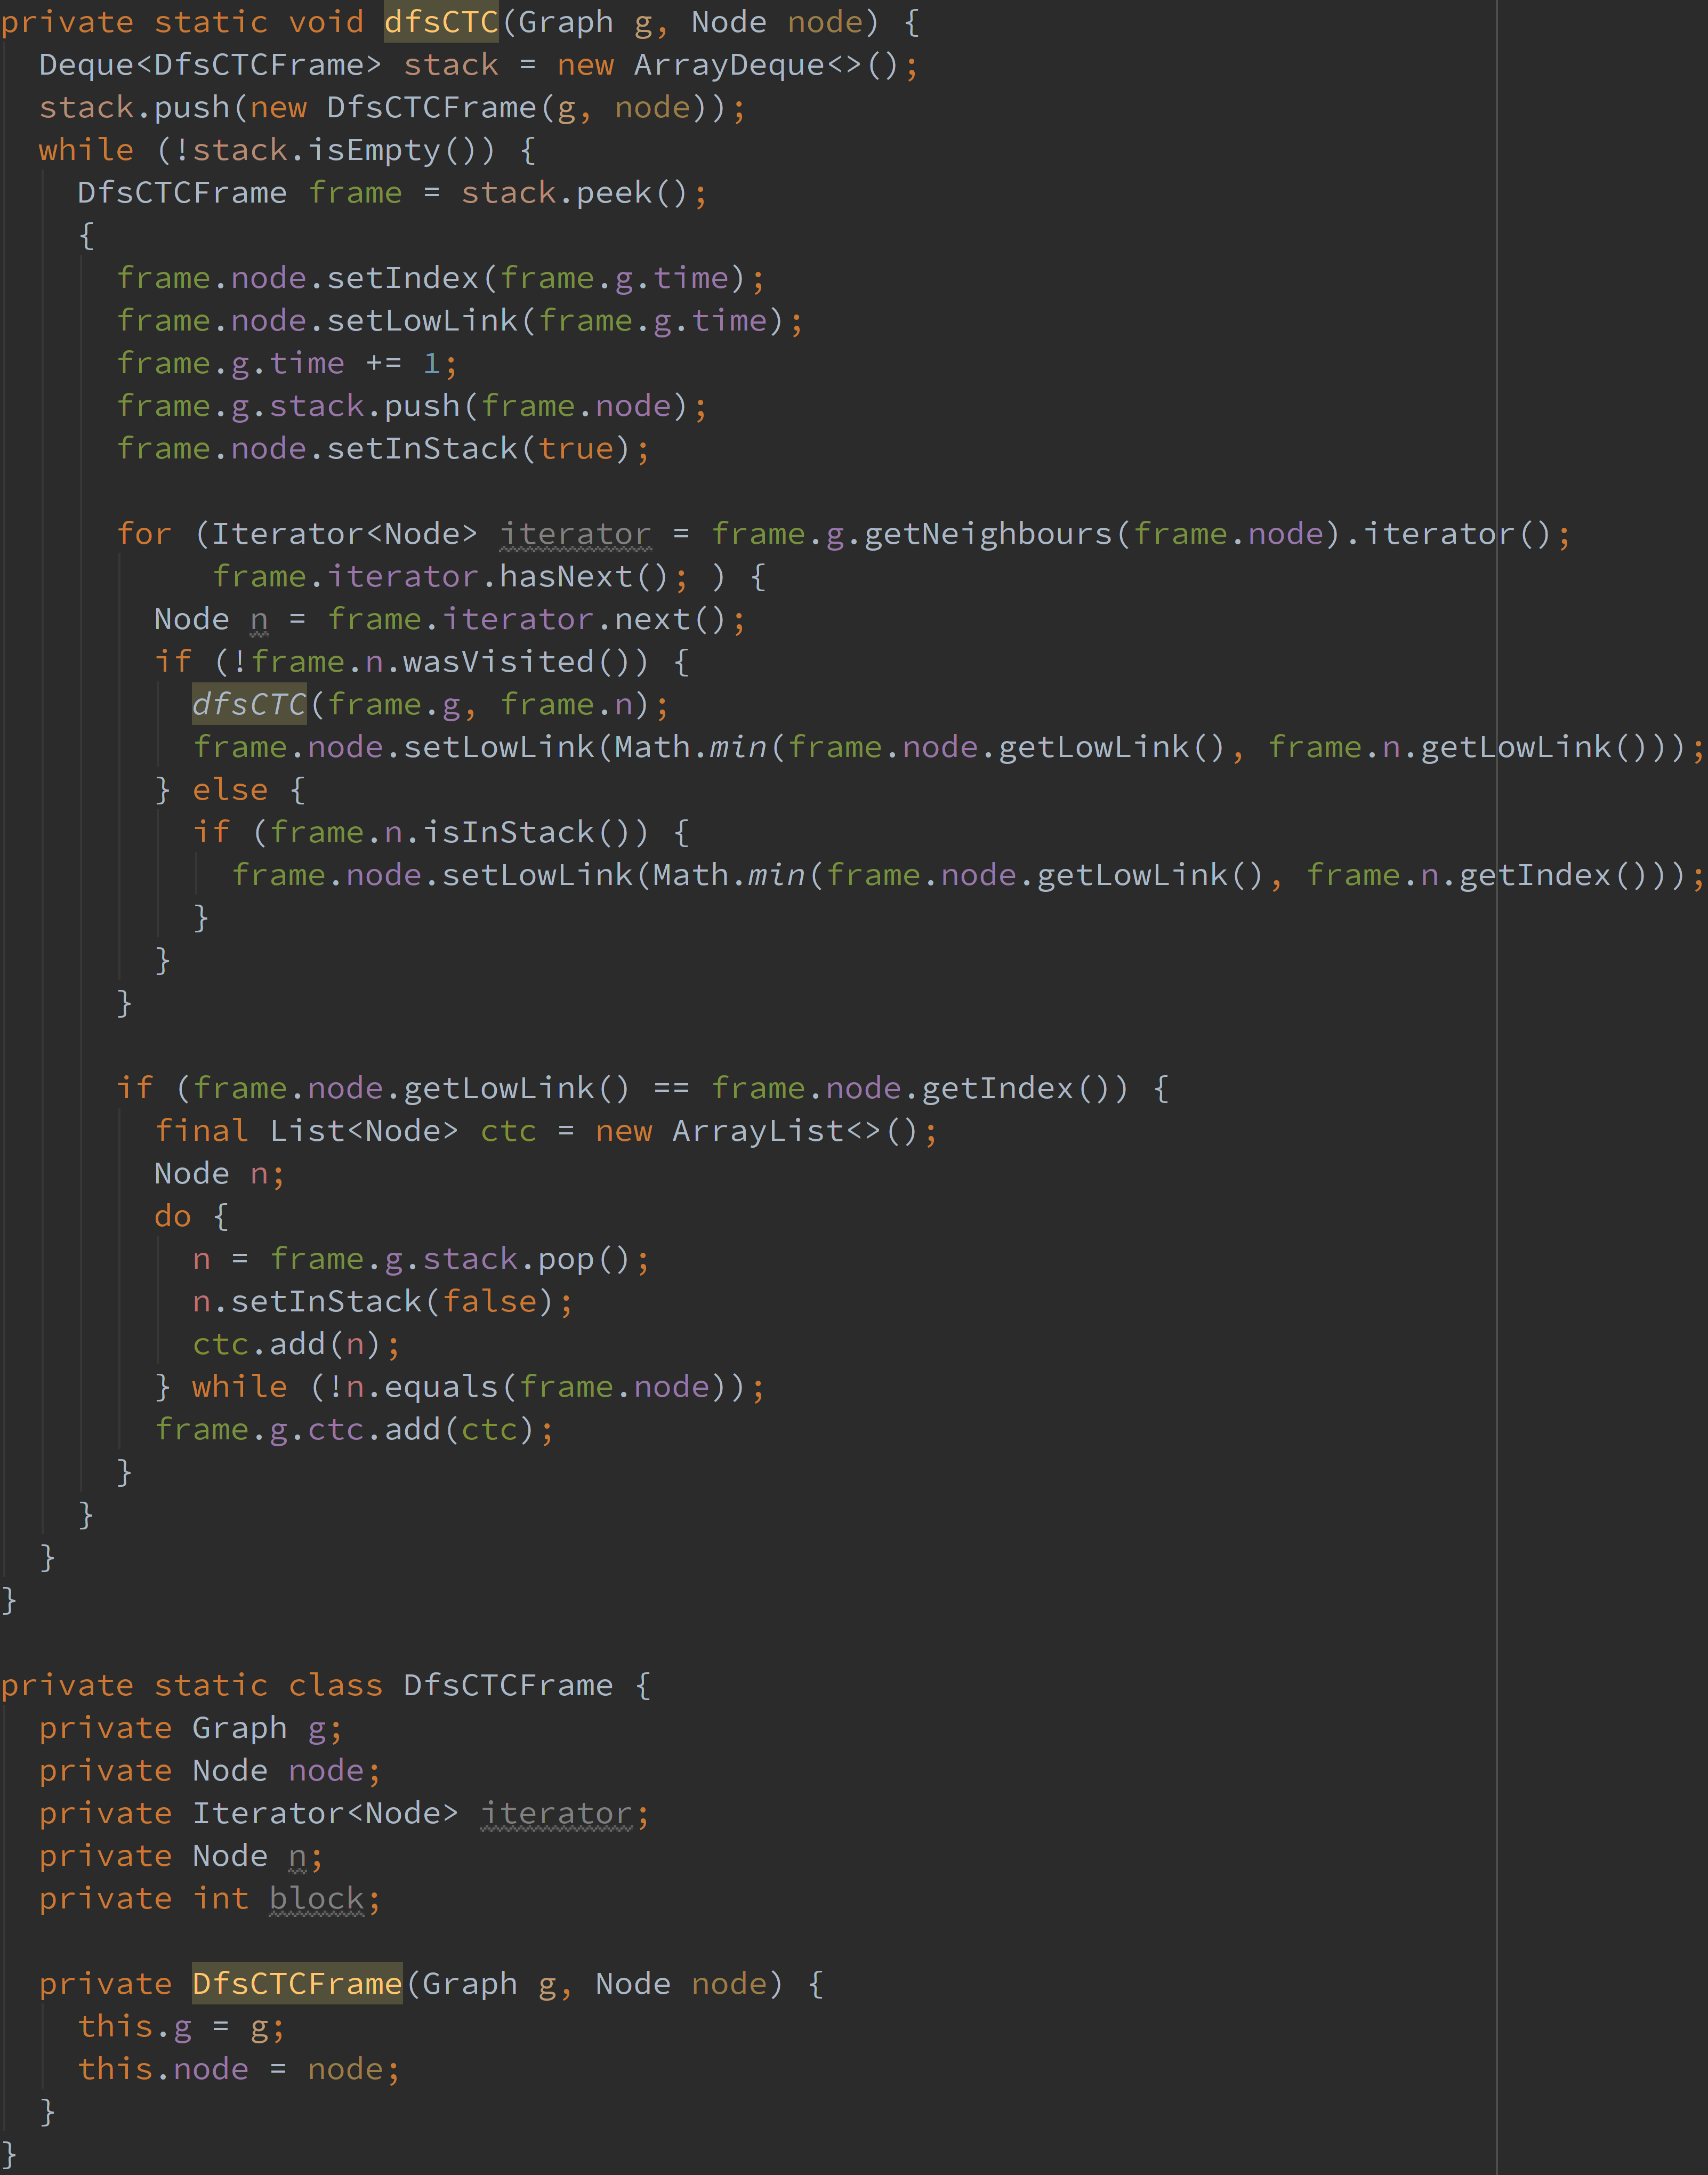
\includegraphics[height=3.7in]{src/img/replace-identifier-after.png}
        \caption{After}
    \end{subfigure}%
    }\\
    \caption{Replacing identifier with frame access \label{img:replace-identifier}}
\end{figure}
\section{Replacing declarations having initializers with assignments}

This pass replaces the local variable declarations in the method body which have initializers with assignments to the
corresponding fields of the \code{frame} object. An example of this pass is provided in
\labelindexref{Figure}{img:replace-declaration}.

\begin{figure}[htb]
    \makebox[\linewidth][c]{%
    \begin{subfigure}[b]{.6\textwidth}
        \centering
        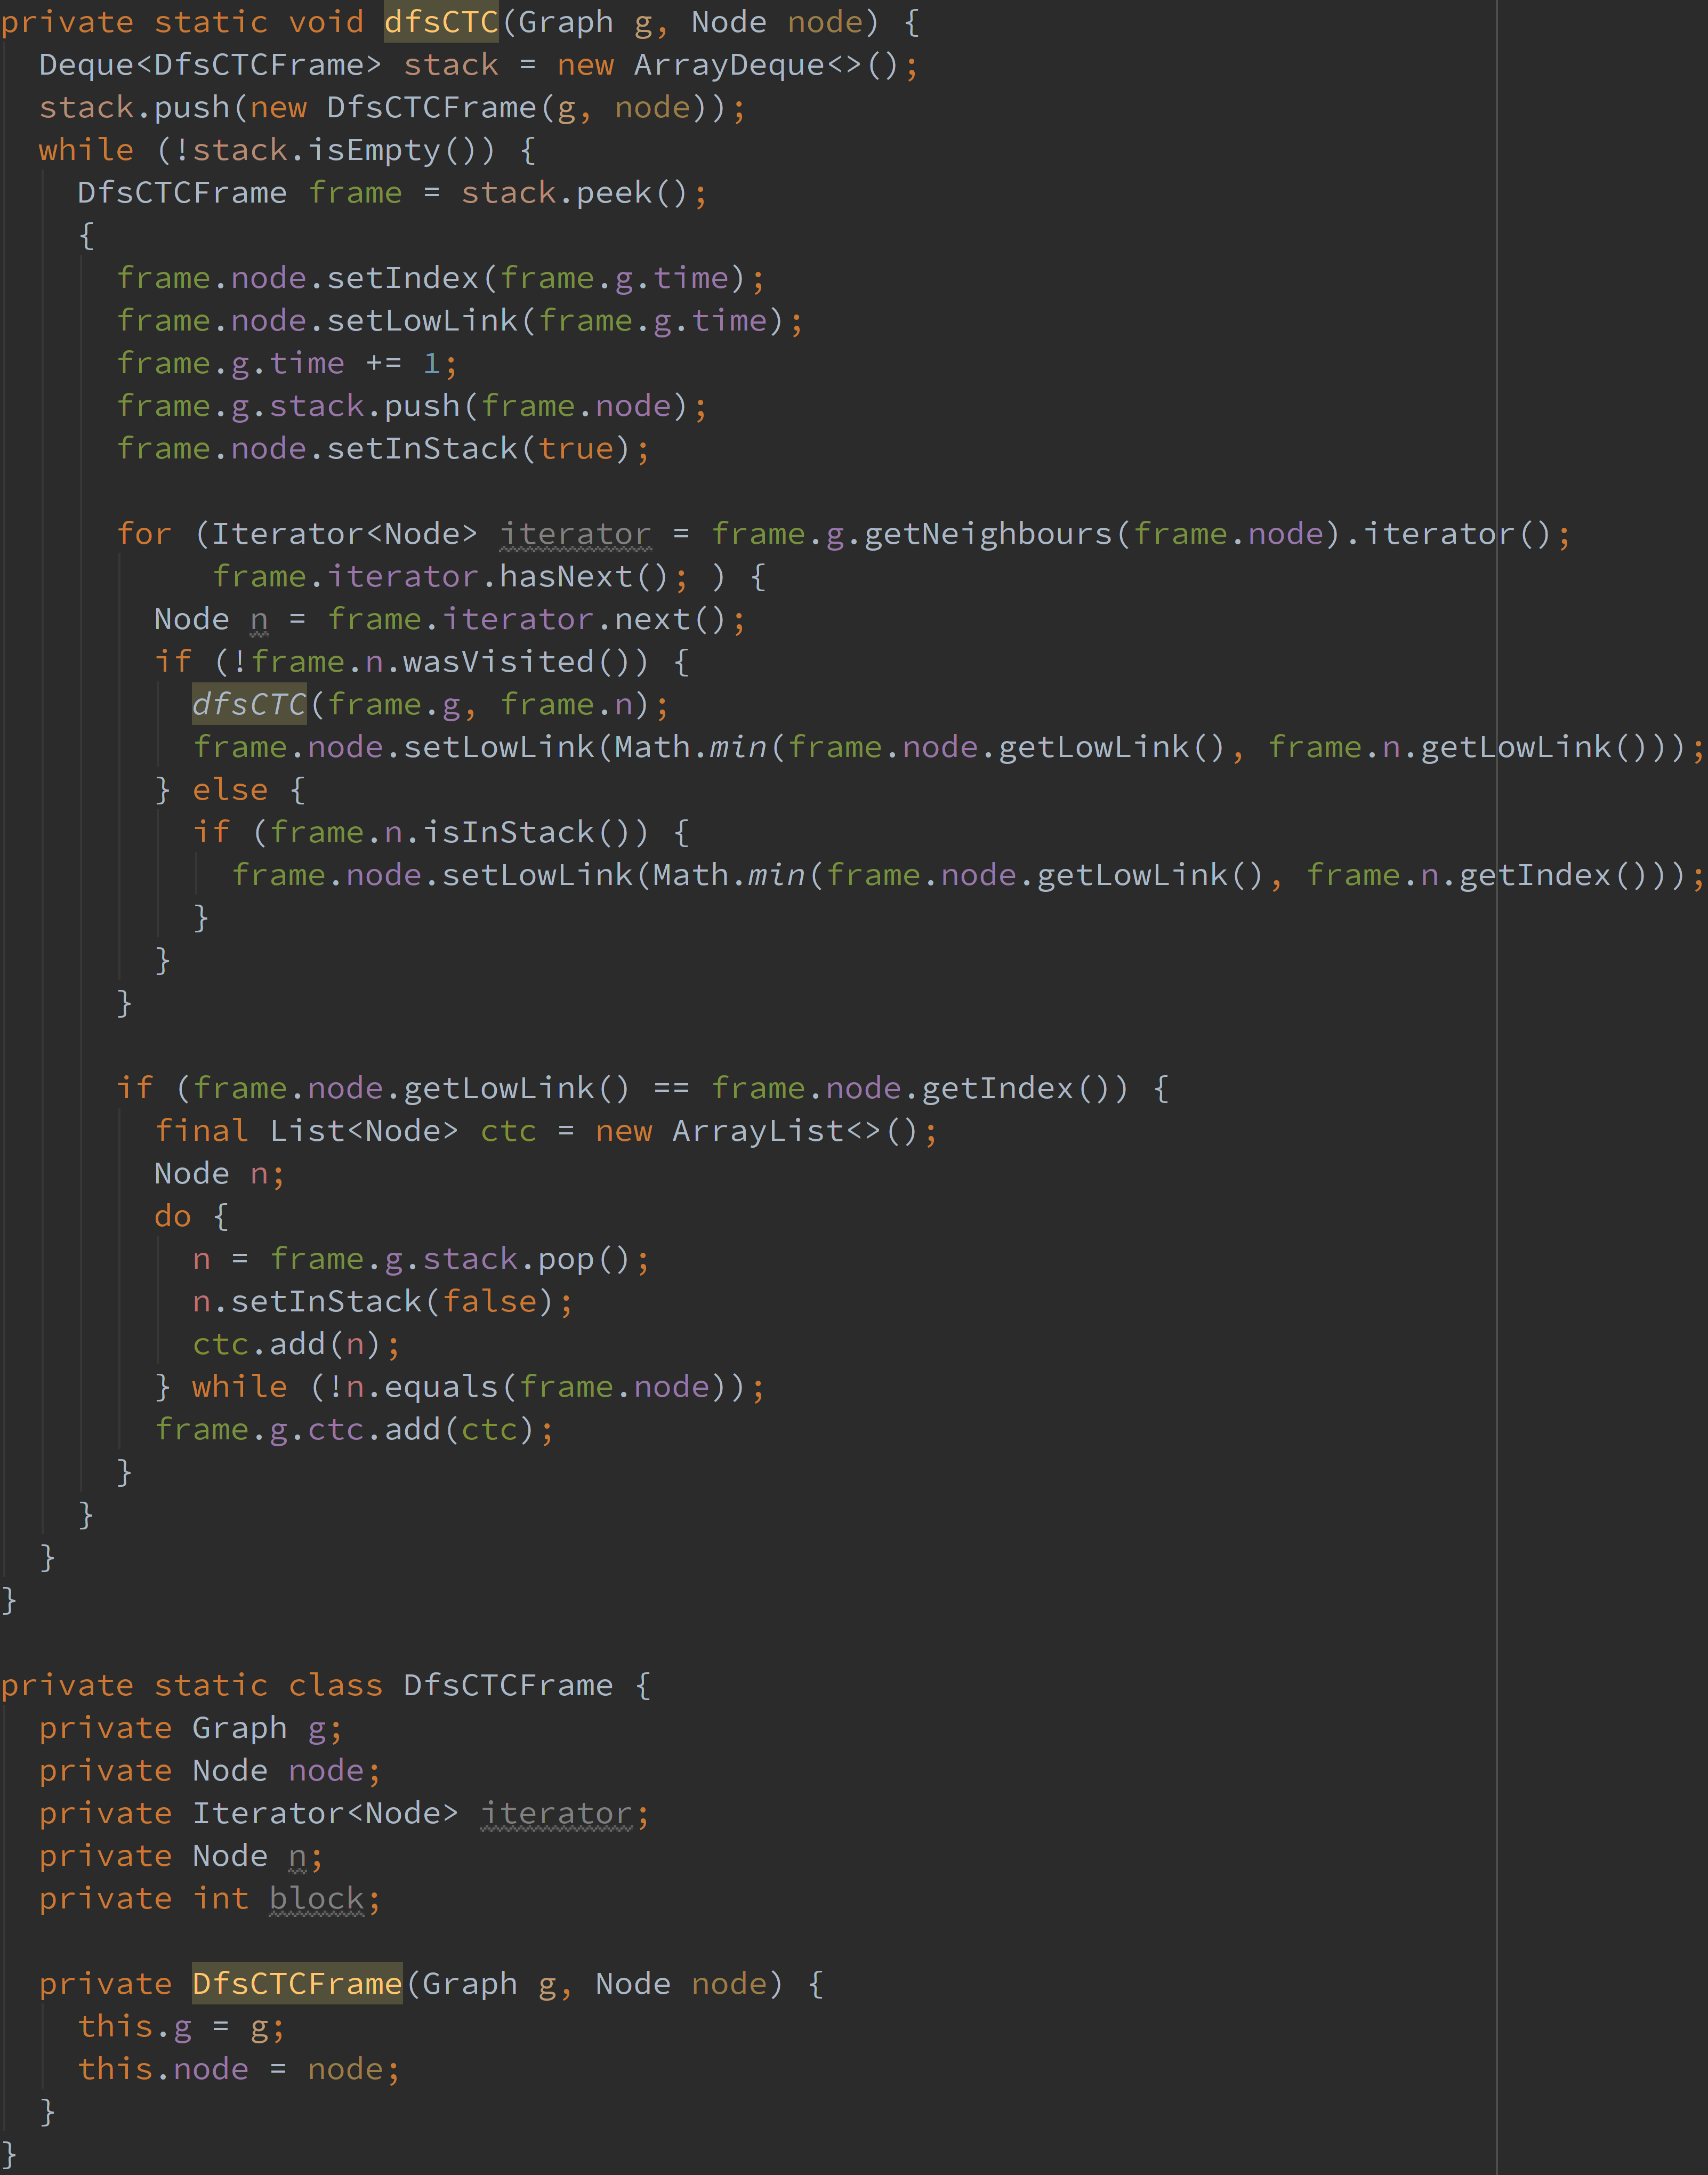
\includegraphics[height=3.7in]{src/img/replace-identifier-after.png}
        \caption{Before}
    \end{subfigure}%
    \begin{subfigure}[b]{.6\textwidth}
        \centering
        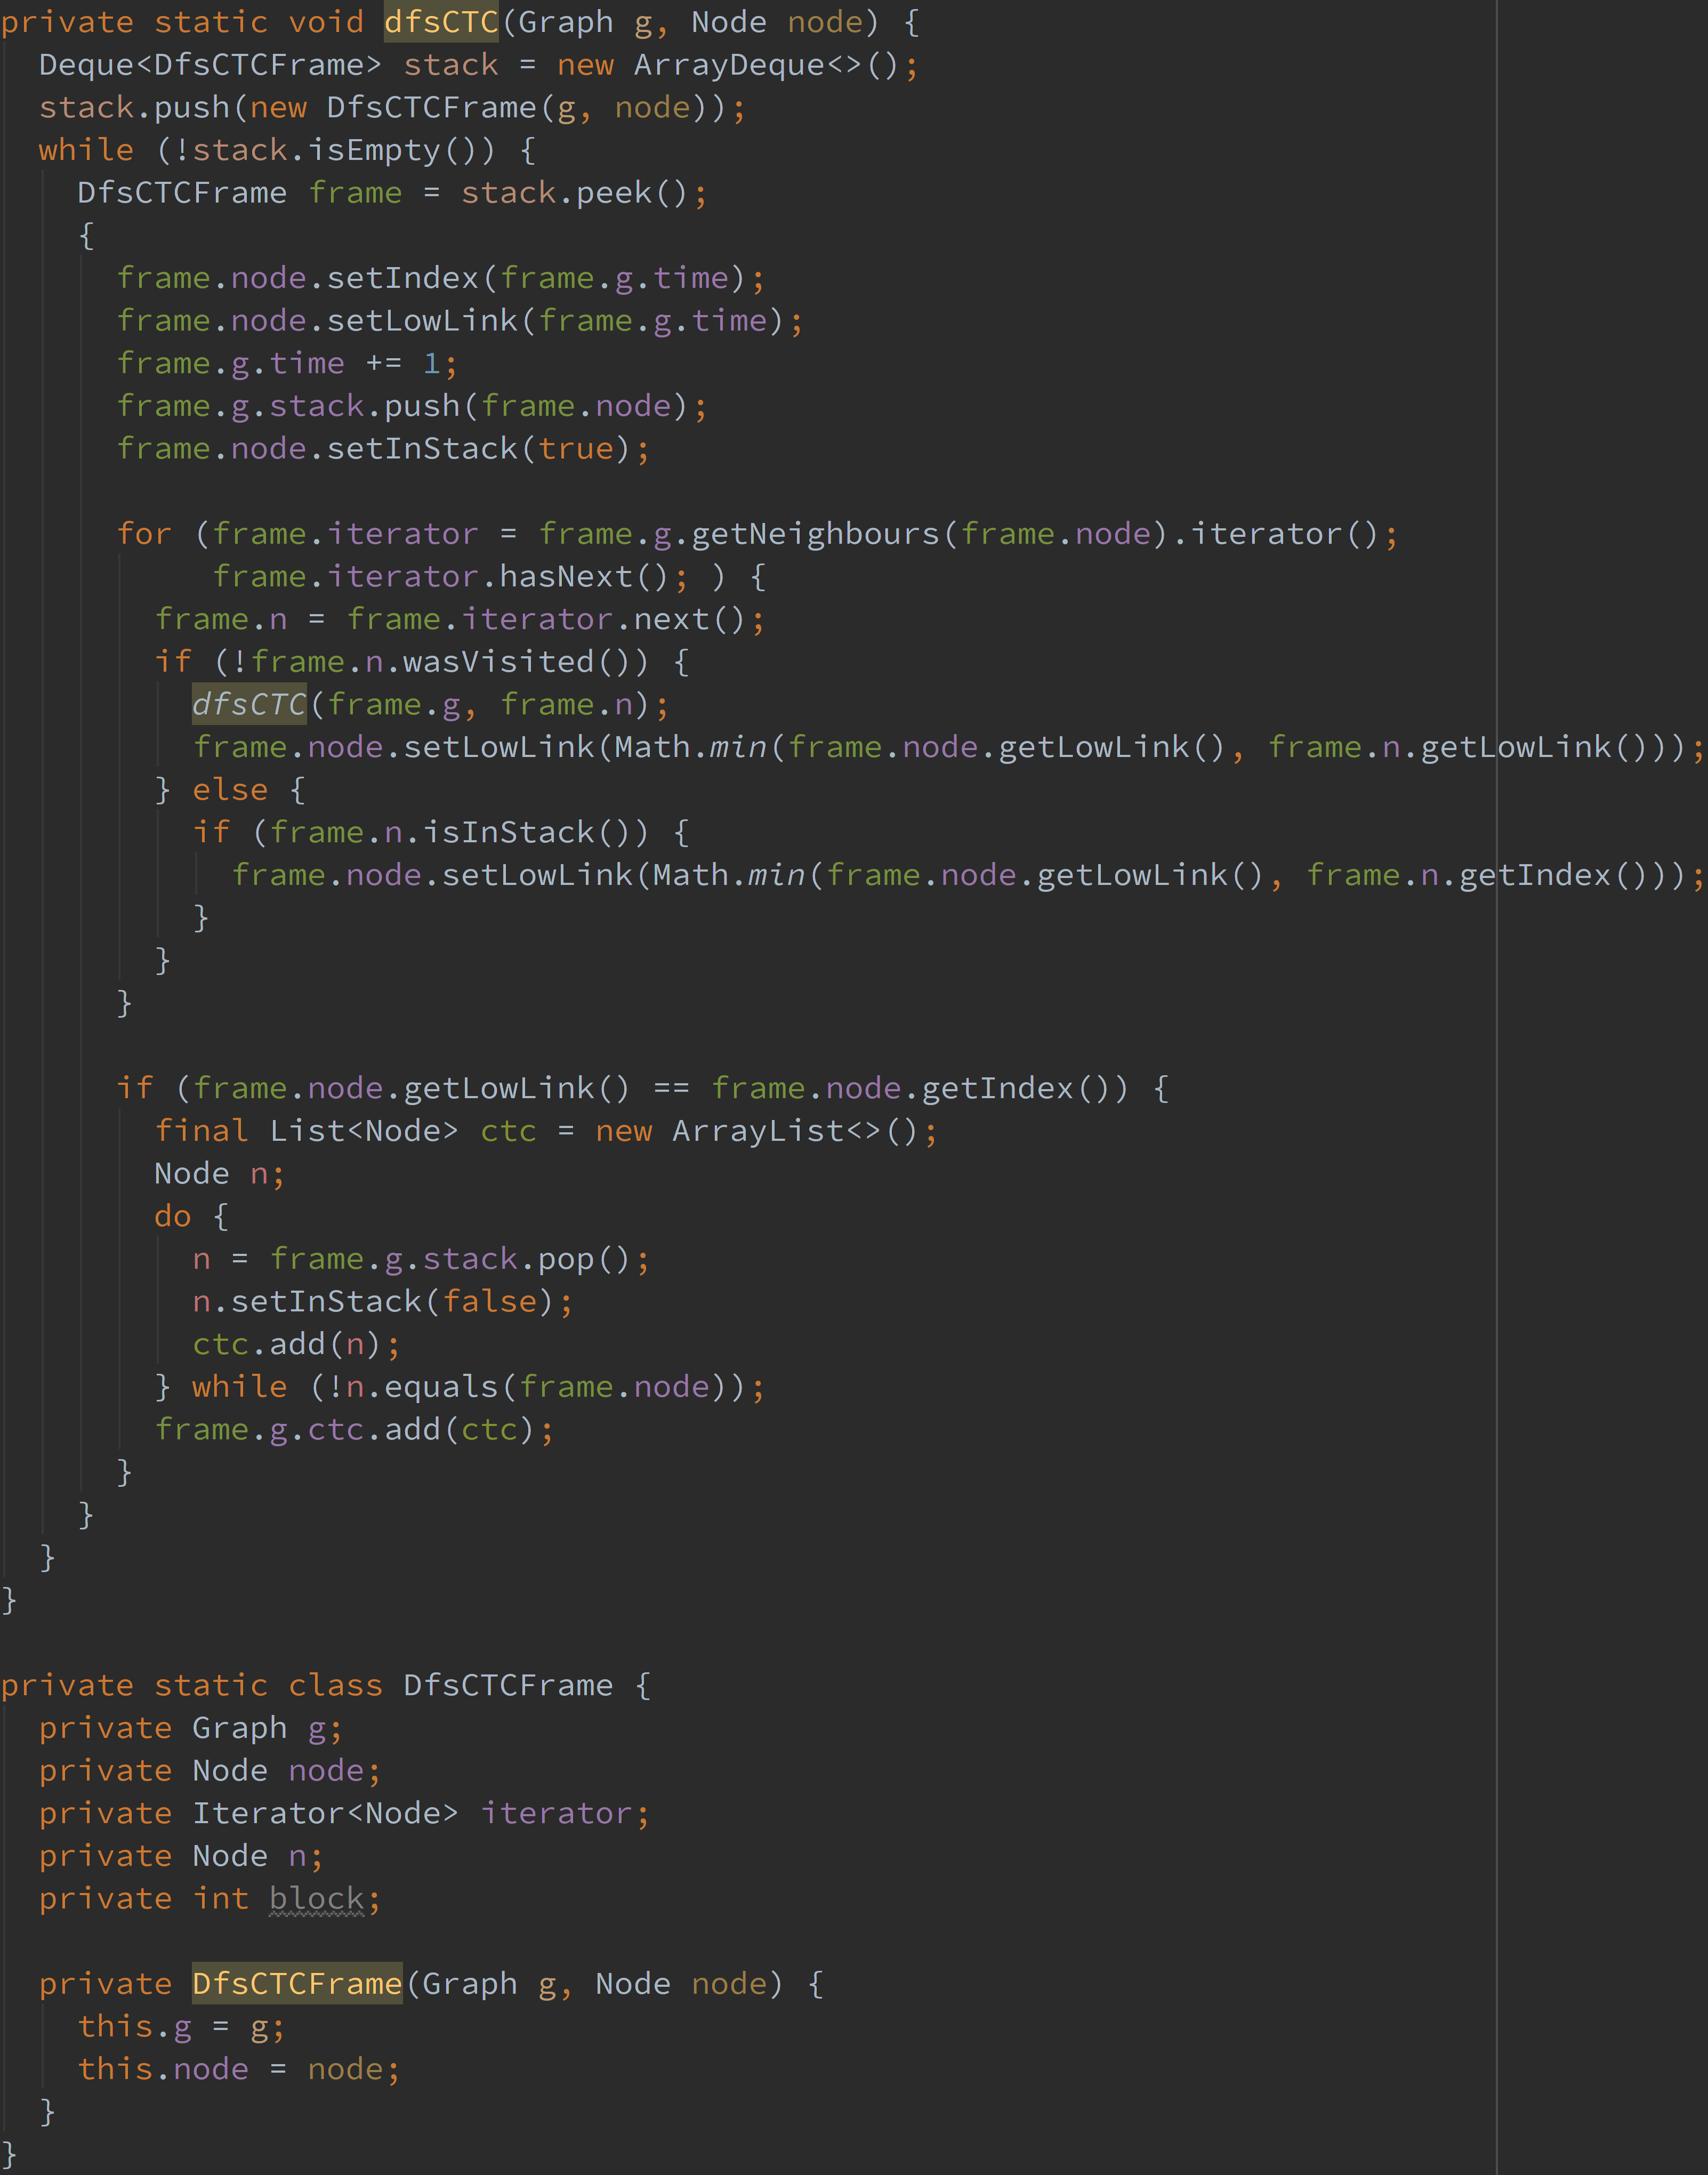
\includegraphics[height=3.7in]{src/img/replace-declaration-after.png}
        \caption{After}
    \end{subfigure}%
    }\\
    \caption{Replacing declarations having initializers with assignments \label{img:replace-declaration}}
\end{figure}
\section{Generating the control flow graph}

The body of the \code{while} statement previously generated will contain a \code{switch} statement, whose body will
contain \code{case}s for each \textit{basic block} in the original body of the method, as defined below.

Because the Java programming language does not provide a \code{goto} statement, there is no direct a way of jumping at
a later point in code (useful when returning from a recursive call to execute the statements after the call). But this
problem can be solved if the code can be broken into \textit{basic blocks}, by generating the control flow graph of the
method body. Each basic block will correspond to a \code{case} in the \code{switch} statement from above. Jumping
between different blocks is possible by using the \code{block} field of the \code{frame} object.

The structure of the CFG (Control Flow Graph) \abbrev{CFG}{Control Flow Graph} presented here is inspired from LLVM
IR\footnote{\url{https://llvm.org/docs/LangRef.html}}.

In this context, a \code{Block} is defined as a list of non-terminal \code{NormalStatement}s terminated by a
\code{TerminatorStatement}.

A \code{NormalStatement} is a wrapper for a \code{PsiStatement}.

A \code{TerminatorStatement} is either a \code{ReturnStatement}, a \code{ConditionalJumpStatement} or an
\code{UnconditionalJumpStatement}.

A \code{ReturnStatement} is a wrapper for a \code{PsiReturnStatement}.

A \code{ConditionalJumpStatement} jumps from the containing \code{Block} to one of two \code{Block}s, based on the
value of a \code{PsiExpression}.

An \code{UnconditionalJumpStatement} jumps from the containing \code{Block} to another \code{Block}.

The list of \code{Block}s for the method body is generated by a \code{JavaRecursiveElementVisitor}, which performs
different operations for each type of \code{PsiElement} encountered. Each \code{Block} has an \code{id} field which
represents the label of its corresponding \code{case}.

The visitor initializes a \code{currentBlock} before visiting the actual body of the method. This is the entry block of
the function. The following subsections present how the visitor processes each type of relevant \code{PsiElement}
encountered.

\subsection{Visiting a \code{PsiCodeBlock}}

The body of a method is represented as a \code{PsiCodeBlock}. The visitor processes each\\
\code{PsiStatement} in the \code{PsiCodeBlock}.

In this context, processing means that if the \code{PsiStatement} contains recursive calls, it
accepts the visitor for further processing. If the \code{PsiStatement} is an instance of \code{PsiReturnStatement}, a
\code{ReturnStatement} wrapper over the \code{PsiStatement} is added to the \code{currentBlock}. Otherwise, a
\code{NormalStatement} wrapper over the \code{PsiStatement} is added to the \code{currentBlock}.

An important last step after processing all the \code{PsiStatement}s in the \code{PsiCodeBlock} of the method is adding
an explicit \code{ReturnStatement} to the \code{currentBlock}, if the return type of the method is \code{void} and the
body does not already contain an explicit \code{return} statement. This is almost always the case because these methods
do not specify a final \code{return} statement, since it is redundant.

\subsection{Visiting a \code{PsiBlockStatement}}
Since the \code{PsiBlockStatement} is merely a wrapper over a \code{PsiCodeBlock}, visiting it translates to processing
the statements of its contained \code{PsiCodeBlock}, just as already specified above.

\subsection{Visiting a \code{PsiMethodCallExpression}}

Given the previous passes and the processing of \code{PsiStatement}s presented above, the visitor actually visits only
recursive calls. These calls appear only as right-hand sides of\\
\code{PsiAssignmentExpression}s or as initializers of \code{PsiVariable}s in\\
\code{PsiDeclarationStatement}s (generated by the \textit{Extracting recursive calls to statements} pass).

The recursive call is transformed in a \code{push} call to the \code{stack}, where the new \code{frame} object is
initialized using the \code{PsiExpression}s provided as arguments to the recursive call. A new \code{Block} is generated
and it is marked as a block appearing after a recursive call, so it will not be considered for inlining by later passes.
Then an \code{UnconditionalJumpStatement} which jumps to the new block is added to the \code{currentBlock}. After this,
the \code{currentBlock} is changed to the new block. The \code{PsiStatement} in which the recursive call appears is
added to the new \code{currentBlock}, but having the recursive call replaced with a \code{PsiExpression} referring to
the \code{ret} variable.
\section{Removing unreachable blocks}

There could be blocks generated in the previous pass which are \textit{unreachable}, meaning that there is no path from
the \textit{entry block} (whose \code{id} is equal to \code{0}) of the control flow graph to these blocks. The entry
block is reachable by default.

This pass visits the control flow graph, which is a directed graph. If the method body does not contain loops, the graph
is acyclic; otherwise, it contains at least one cycle. A breadth-first search algorithm is used to compute the set of
reachable blocks from the entry block of the control flow graph. After the search is finished, the blocks which are not
contained in the set of reachable blocks are removed from the list of all blocks representing the control flow graph.

An example of this pass is provided in \labelindexref{Figure}{img:remove-unreachable}. The blocks with \code{id}s equal
to \code{2} and \code{5} are unreachable from the entry block, so they get removed. Even though the block with \code{id}
\code{2} is reachable from the block with \code{id} \code{5}, it is not reachable from the entry block (with \code{id}
\code{0}), so it still gets removed.

\begin{figure}[htb]
    \makebox[\linewidth][c]{%
    \begin{subfigure}[b]{.6\textwidth}
        \centering
        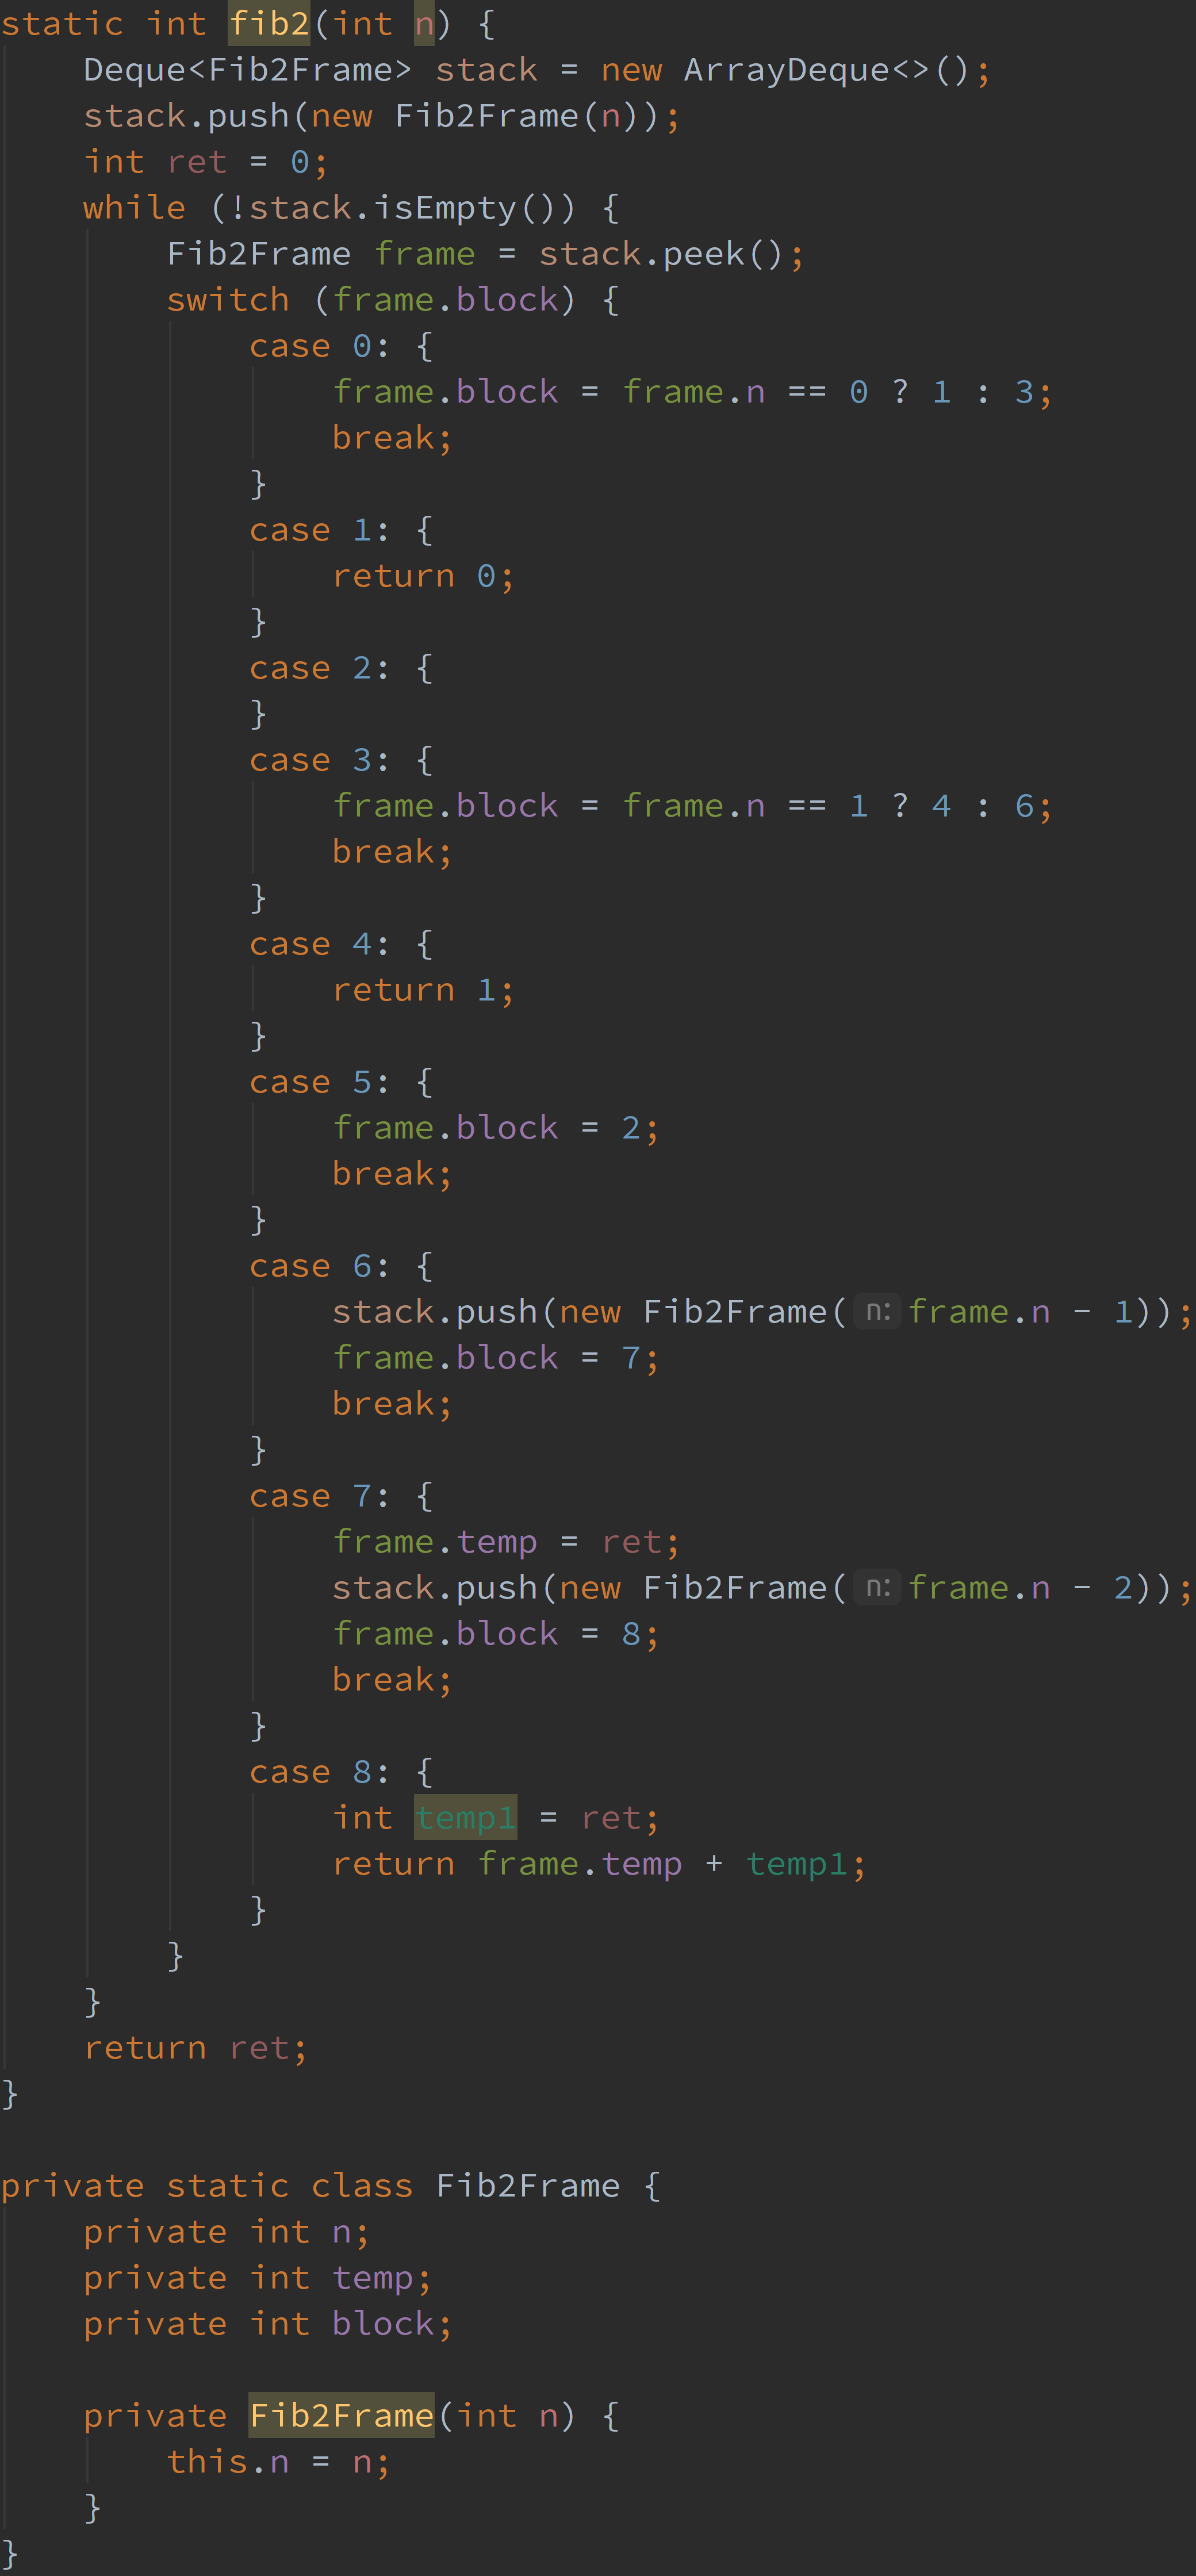
\includegraphics[height=5in]{src/img/blocks-after.png}
        \caption{Before}
    \end{subfigure}%
    \begin{subfigure}[b]{.6\textwidth}
        \centering
        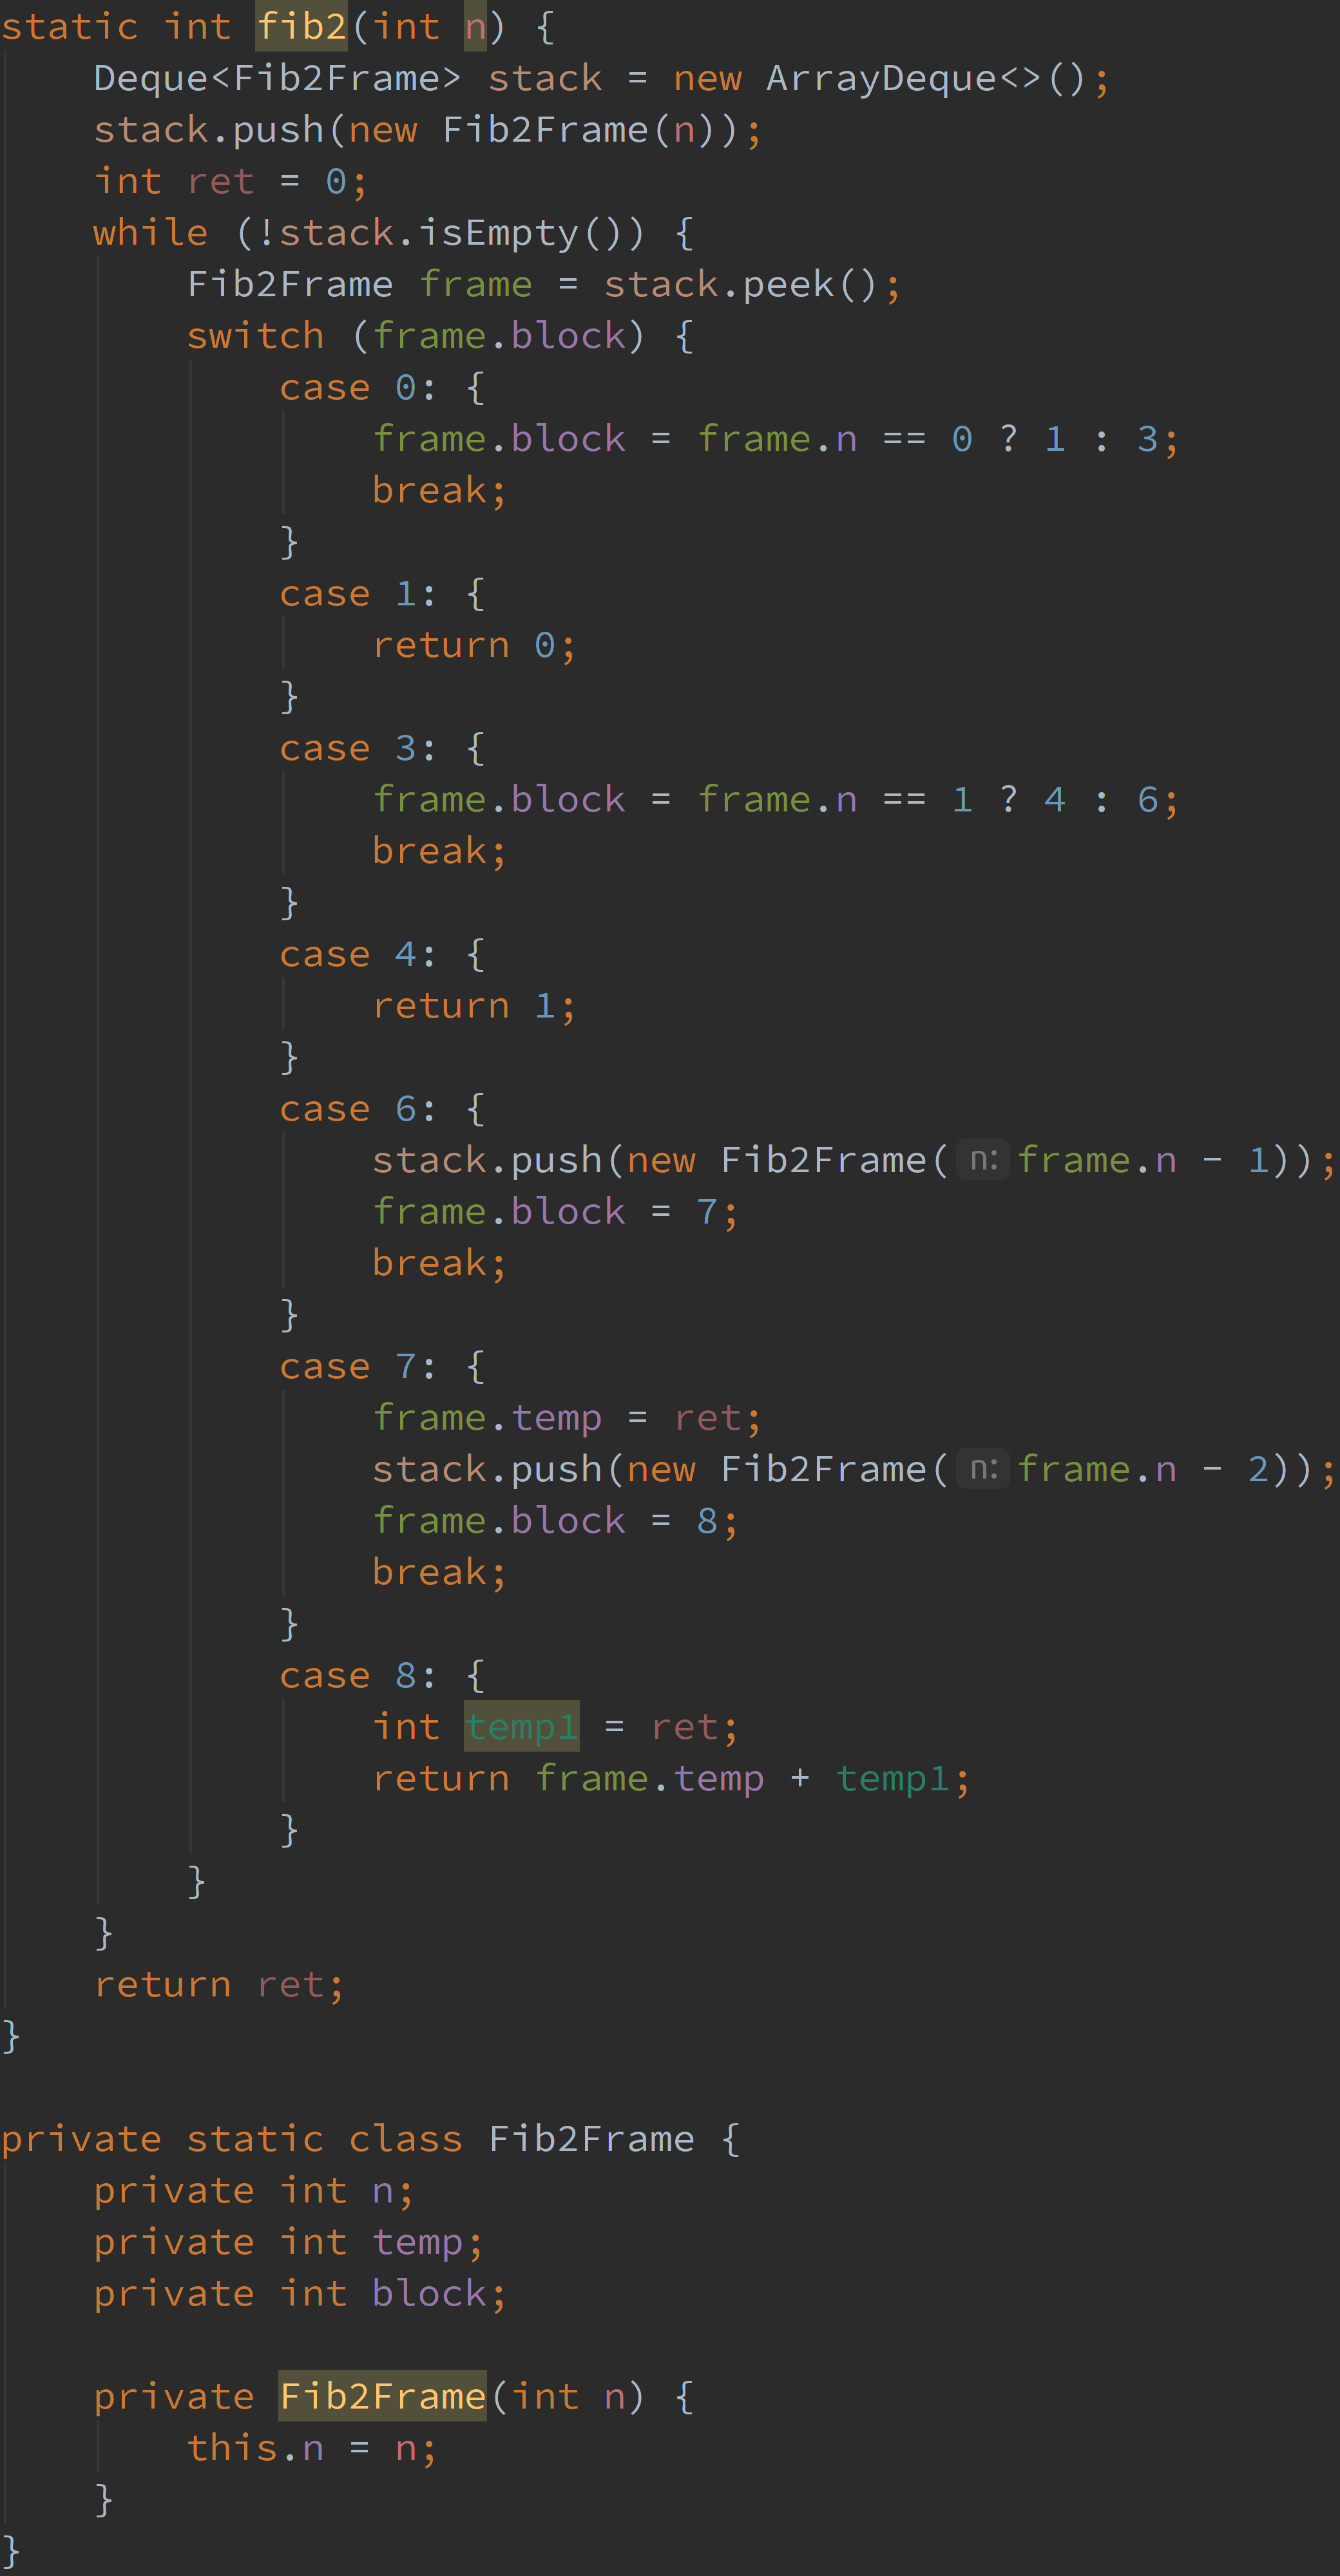
\includegraphics[height=4.464in]{src/img/remove-unreachable-after.png}
        \caption{After}
    \end{subfigure}%
    }\\
    \caption{Removing unreachable blocks \label{img:remove-unreachable}}
\end{figure}